% About Unity

\section{External Resources}
The Design Review application was implemented by using several pre-made assets.
When the application is started user is positioned into a oiltank model, which was provided by DNV GL. 
This model is of high fidelity and was originally developed for the DNV GL Survey Simulator, an application to train surveyors.

\begin{figure}%[h!] %[H]
	\frame{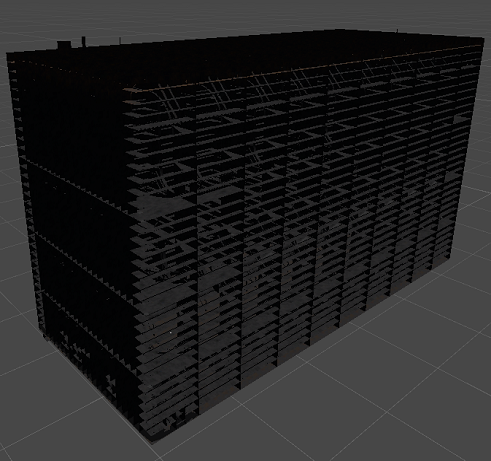
\includegraphics[width=0.5\linewidth]{pictures/screenshots/tank_back.png}}
	\frame{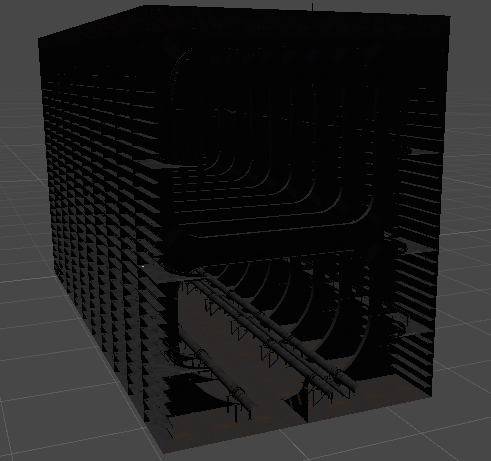
\includegraphics[width=0.5\linewidth]{pictures/screenshots/tank_half_profile.png}}
	\caption[The Oil tank model]{The Oil tank model from the outside}
	\label{fig:tank_outside}
\end{figure} 

The application also makes use of several "best practice" assets from Leap Motion, Oculus VR and SteamVR to ensure that these devices function
as optimally as possible. From Leap Motion the \texttt{LeapHandController} is utilized, which is a prefab (gameObject), with several important scripts attached to
it. Leap motion provided hand models are also being used, which was provided from the Leap Motion Hands-module. More specifically 
the \texttt{RiggedPepperCutHands} were used, but any other of the hand models could be used as easily.

From Oculus VR two prefabs is used. The first is \texttt{OVRCameraRig}, which is the recommended camera setup for using the Oculus Rift HMD. This 
prefab sets several important settings to ensure that both the head tracking and visual performance is as optimal as possible. The 
second prefab which is used is one called the \texttt{GazePointerRing}. This was showcased in a demo unity implementation by OculusVR
and is essentially a cursor that exist in the game world a fixed length in front of the user. As regular crosshair (which are drawn directly on the screen space)
isn't allowed in VR (more about this later), the \texttt{GazePointerRing} serves as a crosshair. 
From SteamVR the \texttt{[CameraRig]} prefab is used, which essentially does the same configurations as the \texttt{OVRCameraRig} does, but with the HTC Vive HMDs in mind.

The Design review application also makes use of Hover UI Kit, an open source project for creating VR/AR-enabled, customizable and dynamic user interfaces. 
This kit was vital in rapidly prototyping a gesture-enabled menu and a virtual keyboard to the annotation forms.

% \section{The architecture}
\begin{figure}%[h!] %[H]
	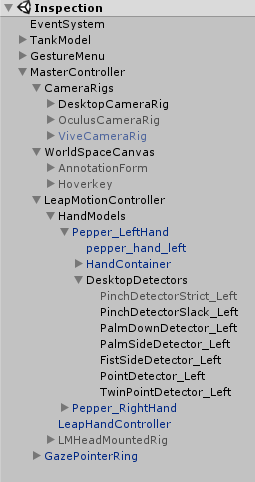
\includegraphics{pictures/unity_hierarchy.png}
	\caption[The Unity project hierarchy of the Design Review Application]{The Unity project hierarchy of the Design Review Application}
	\label{fig:unity_hierarchy}
\end{figure} 

The Unity project has four top-level game objects, as visible in \ref{fig:unity_hierarchy}. 
These will be covered by their own sections, with subsections detailing their important child game objects where appropriate.

% In short terms EventSystem is responsible for processing and handling events and input actions in the scene.
% The TankModel game object contains several child objects that together make up the oiltank-model.
% GestureMenu contains the menu, all its interactable buttons and several scripts.
% The MasterController . 

\section{The Master Controller}
The \texttt{MasterController} game object represents the player model and contains many of the most important game objects, in addition to
holding many key scripts. The \texttt{MasterController}'s transform, with its position, rotation and scale, represents the user's position and orientation, 
and every child object of \texttt{MasterController} will have a position, rotation and scale that is relative to its own. This ensures
that e.g.~the camera will always "follow" the user. Because this game object is so essential, we will cover several important components and
child objects in the following sections.

\begin{figure}%[h!] %[H]
	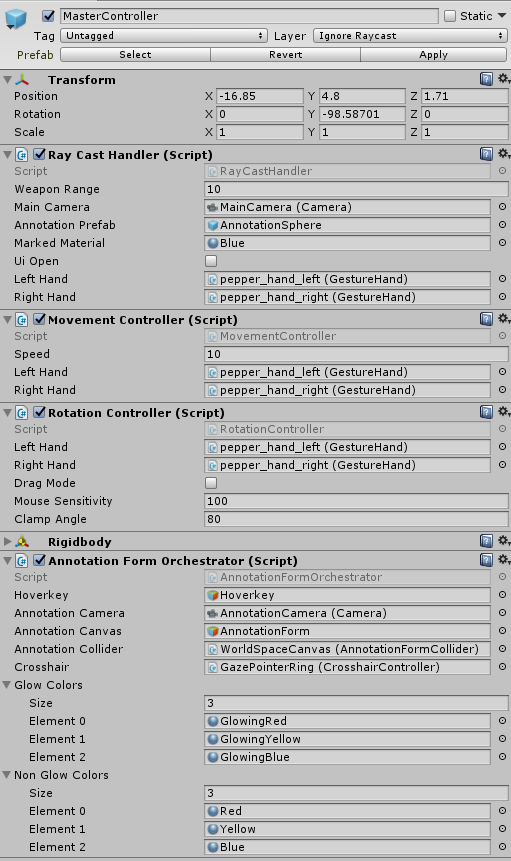
\includegraphics{pictures/unity_inspector.png}
	\caption[The \texttt{MasterController} components]{The \texttt{MasterController} components seen in the Unity Inspector view.}
	\label{fig:unity_inspector}
\end{figure} 

\section{The Camera Rigs}
The \texttt{CameraRigs} game objects holds three different game object, which each represents its own camera-setup: \texttt{DesktopCameraRig}, which is meant to be used
without virtual reality, \texttt{OculusCameraRig}, meant to be used with Oculus Rift HMDs, and \texttt{ViveCameraRigs}, meant to be used with the HTC Vive. 
While the desktop rig uses one main camera, the virtual reality rigs (i.e the Oculus and Vive rigs) utilizes two main cameras (one per eye).
These are slightly offset, by about the same length as the real-world distance between two eyes, and rendered separately.
The camera rigs all utilize a separate camera for rendering annotation objects in the scene, while the main camera(s) (one for desktop, two for VR), 
renders the rest. This is done by:

\begin{enumerate}
	\item Placing the annotation objects in the scene on a different rendering layer than the rest of the objects (called the annotation-layer).
	\item Have the annotation-camera only render objects on this layer.
	\item Have the main camera(s) render the other layers.
	\item "Combining" the results into the resulting frames the user will see.
\end{enumerate}

By rendering these two categories of layers independently we get some flexibility and options with regards to how to present the annotations.
This will be discuss more in depth in the \ref{sec:annotations} section.

For the application to run successfully one of these rigs should be enabled, while the other two should be disabled.
This can be done by switching between the three rigs in the dropdown-menu named Rig, which is present on the \texttt{CameraRigs} game object itself and
implemented in the \texttt{CameraRigSetup} script. In addition to ensuring that only the correct rig is enabled, 
the \texttt{CameraRigSetup} script also does several other operations. One of these is ensuring that the field of view is set to 60 degrees if the desktop rig 
is selected, as this can wrongfully be set to a HMD's value if a HMD is connected to the computer. When a virtual reality rig is used the field of view is 
set automatically by the HMD software. Another thing done by the script is to decide wheter a two dimensional crosshair/cursor should be drawn on the screen space
(in case of the desktop rig), or if a three dimensional crosshair/cursor (i.e the \texttt{GazePointerRing}) should be drawn in the world space. 


\section{The World Space Canvas}
The \texttt{WorldSpaceCanvas} is a canvas object, which in Unity serves as a container for other user interface elements, such as buttons and input fields, 
and is rendered in world space. It is thus diegetic and exists there like other 3D objects.

In applications that don't utilize virtual reality, canvases and other UI elements are usually non-diegetic (i.e they don't exist within the game world), 
and in 2D and drawn directly to the screen space (as opposed to world space) using x- and y-coordinates.
With this approach one can specify e.g.~a position by its x- and y-coordinate, where \{0, 0\} usually represents the top-left of the display.
This changes in virtual reality applications, as the user's eyes are unable to focus on the screen space. An analogy to this would be to 
ask the user to read a letter while holding it 2-3 centimeters from their eyes. Because of this, elements appearing on the screen space is not rendered
in unity while running it with the virtual reality SDKs. 

\begin{figure}%[h!] %[H]
	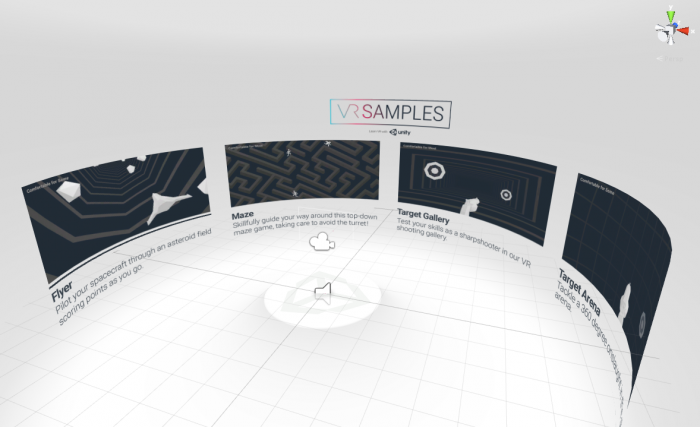
\includegraphics[width=\linewidth]{pictures/unity_vr_menu.png}
	\caption[An example of world-space (diegetic) user interfaces]{An example of world-space (diegetic) user interfaces~\citep{Unity}.}
	\label{fig:unity_vr_menu}
\end{figure} 

Another reason why the canvas is rendered in world space, and also the reason why this is the case in desktop mode, is because of our touch interaction.
To enable the user to click on buttons using his or her hands, the user interface must also exist in world-space so a collision can occur between the desired 
button and the hand models (that mimic the users hand). 

\texttt{WorldSpaceCanvas} is thus rendered in the world space, and is always positioned 0.8 unity meters (i.e the virtual representation of a meter in unity) 
in front of the user. The game object is thus always in the center of the camera, but is only visible and enabled when the user is editing an annotation. 
One issue with this approach is "clipping", i.e that the annotation form visually collides with another object (e.g.~the tank model or an annotation sphere) thus
obstructing it from view. To combat this \texttt{WorldSpaceCanvas} has a box-shaped collider component, which covers the canvas as well as the area between the canvas and the camera, 
and a script called \texttt{CanvasCollider}, which keeps track of objects that's within the collider component. When the user wish to edit an annotation, and the 
\texttt{AnnotationForm} and \texttt{Hoverkey} becomes active, the objects within the canvas' collider is disabled, thus hiding objects that could potentially
obstruct the whole, or parts of, the canvas. The objects are enabled again once the users is done editing the annotation (i.e when the user clicks "submit", "cancel" or "delete").

\begin{figure}%[h!] %[H]
	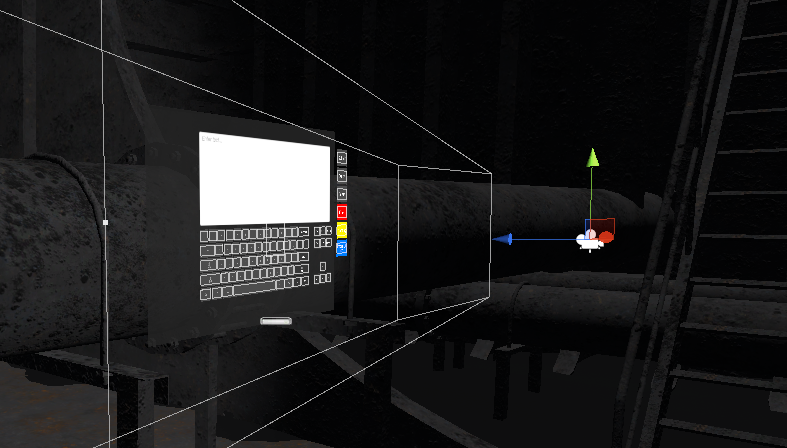
\includegraphics[width=\linewidth]{pictures/screenshots/canvas/worldspacecanvas_scene.png}
	\caption[The \texttt{WorldSpaceCanvas} as seen in the Unity Scene View]{The \texttt{WorldSpaceCanvas} as seen in the Unity Scene View.}
	\label{fig:worldspacecanvas_scene}
\end{figure} 

\begin{figure}%[h!] %[H]
	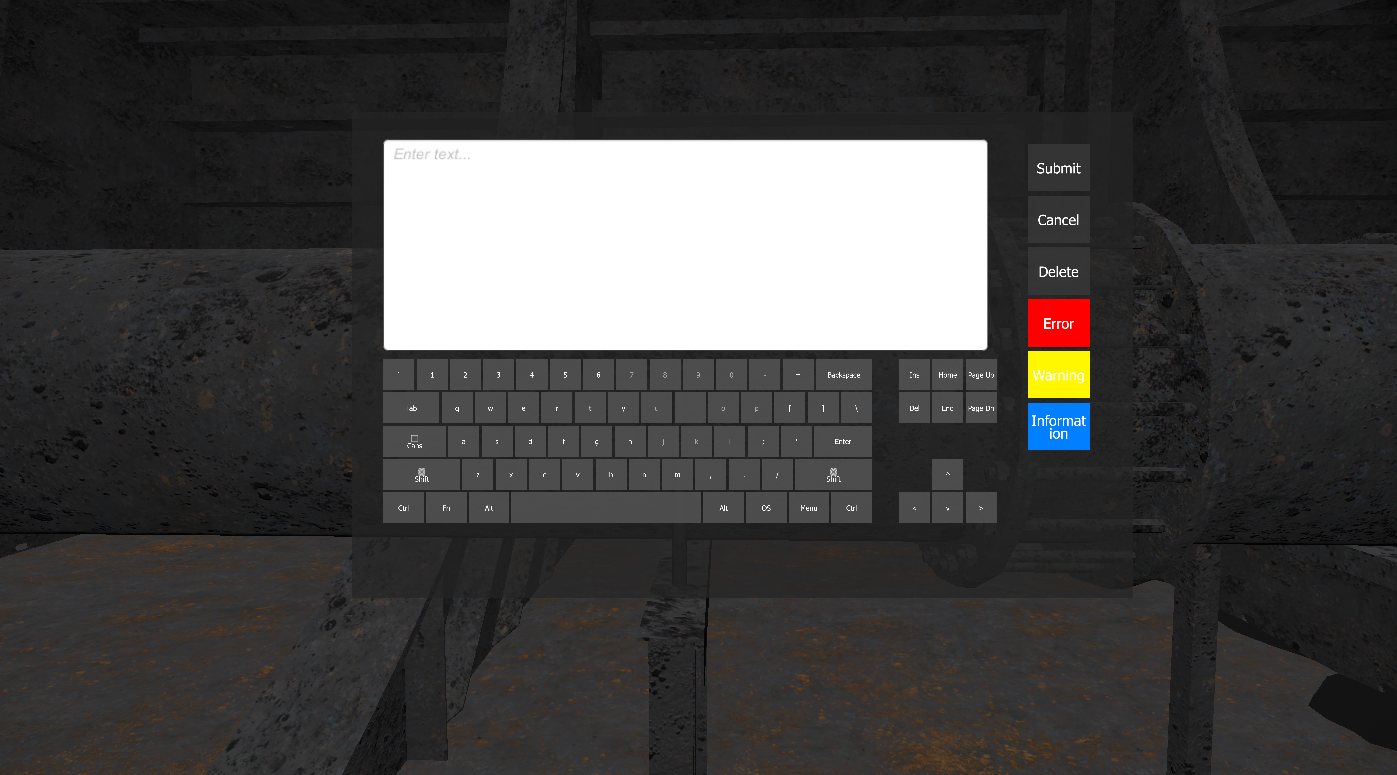
\includegraphics[width=\linewidth]{pictures/screenshots/canvas/worldspacecanvas_ingame.png}
	\caption[The \texttt{WorldSpaceCanvas} as seen in the Unity Game View]{The \texttt{WorldSpaceCanvas} as seen in the Unity Game View.}
	\label{fig:worldspacecanvas_ingame}
\end{figure} 

The \texttt{WorldSpaceCanvas} has two child game objects: \texttt{AnnotationForm} and \texttt{Hoverkey}. 
\texttt{AnnotationForm} currently only contains a inputfield-object and a background rectangle, but can in future iteration grow to 
contain other user interaction elements. The \texttt{Hoverkey} game object represents the touch keyboard and is part of the HoverUI-kit.
In addition to the keyboard six other similar buttons are also present: Submit, Cancel, Delete, Error, Warning and Information (see \ref{fig:worldspacecanvas_ingame}).

\section{The Leap Motion Controller}
The \texttt{LeapMotionController} game object contains objects related to the Leap Motion device and gesture recognition and consist primarily of the hand models, necessary 
scrips and detectors. In the game object \texttt{HandModels} there is one object-representation of the left hand, called \texttt{Pepper\_LeftHand}, and one for the 
right hand, called \texttt{Pepper\_RightHand}. These objects have their own hand models (as there needs to be different models for the left and right hand) and their 
own detector objects (as a detector can/should only observe one hand). Each "hand" thus have its own list of detectors called \texttt{Detectors}. 
These are the definition and implementation of the gesture scheme that were discussed in \ref{sec:gesture_design}. In addition to detectors, each
hand also have its own instance of the \texttt{GestureHand} class, which is an important component to keep track of hand states and resources, and
it exposes utility function to other classes. 

\section{The GestureHand Class}
The \texttt{GestureHand} class is assigned as a component to each hand object, and contain several important variables.
\begin{itemize}
	\item \texttt{bool isLeftHand} - Keeps track of whether this instance belong to the left or the right hand.
	\item \texttt{GameObject handModel} - A reference to the unity game-object that contains the handModel this gesturehand instance is relevant for.
	\item \texttt{Material[] handMaterials} - An array of different material for the hand model. These are swapped between when e.g.~a certain gesture is brecognized and tracked.
	\item \texttt{GestureHand otherHand} - A reference to the other GestureHand-instance. For the lefthand GestureHand-instance this variable thus point to the right hand GestureHand
			hand-instance.
	\item \texttt{GameObject detectors} - A reference to the gameobject that hold/is parent of this hands detectors.
	\item \texttt{bool combineGestures} - Keeps track of whether the user is using a combined XYZ axis gesture scheme or if these movement gesture are kept separate (see \ref{sec:combined-movement}).
	\item \texttt{Vector gestureOriginPosition} - Holds the x-, y- and z- coordinates of the palm when the current gesture was recognized.
	\item \texttt{HandState handState} - Holds one of several HandState enum values that represent the hand state. This variable has one of the following enum values:
			NONE = 0, PINCH = 1, PALM\_DOWN = 2, PALM\_SIDE = 3, FIST = 4, SINGLE\_POINT = 5, DOUBLE\_POINT = 6 or DISABLED = 7 (see \ref{tab:handstates}).  
\end{itemize}

\begin{table}[]
\centering
\label{tab:handstates}
\begin{tabular}{p{1cm}| p{3.5cm} | p{6cm}}
	\textbf{ID} &  \textbf{Variable name} &   \textbf{Implication} \\\\
	0 & NONE & No gesture is being performed. \\\\
	1 & PINCH & User can rotate by the y- and z-axis \\\\
	2 & PALM\_DOWN & User can move along the y-axis.  \\\\
	3 & PALM\_SIDE & User can move along the x-axis.  \\\\
	4 & FIST & User can move along the z-axis.  \\\\
	5 & SINGLE\_POINT & User is placing/has placed point-annotation.  \\
	6 & DOUBLE\_POINT & User is placing/has placed object-annotation.  \\
	7 & DISABLED & The detectors are disabled and no gesture and hand state can be achieved before enabling them.  
\end{tabular}
\caption{The \texttt{GestureHand} class' hand states}
\end{table}

The \texttt{GestureHand} class also contains several important functions that are called when a certain gesture is activated or deactivated.
\texttt{void ActivateGesture(int gestureCode)} is called by a detector when it becomes active, i.e when its criteria are met and the gesture it represent is recognized.
It then signals the \texttt{GestureHand} class with its code/signature so \texttt{GestureHand} knows which detectors called it.
If a pinch gesture is detected by the left hand pinch detector the left hand \texttt{GestureHand} class' \texttt{ActivateGesture} is thus called with the argument "1".
From a design standpoint one should be able to send the Handstate.PINCH enum as a value, but then this function wouldnt be exposed in the Unity Inspector interface (which
only seem to accept primitive or built-in argument types). 

Once this function is called it sets the hand state to the value of the gestureCode, sets the gesture origin position and switches the hand materials.
Hand material switches is done by assigning the material at index \texttt{gestureCode} in the \texttt{handMaterials} list to the hand model, so 
if a pinch gesture is a performed the hand model is assigned the material at \texttt{handMaterials[1]}. The HandState enums and the hand material list thus 
follow the same sorting order. 

The \texttt{GestureHand} class also has the function \texttt{void DeactivateGesture()}, which is called by a detector when it becomes deactivated. 
This function simply resets the hand state by setting it to HandState.NONE (NONE = 0) and assign the material at \texttt{handMaterials[(int) HandState.NONE]} (i.e 0) to the
handmodel. \texttt{GestureHand} also contains the functions \texttt{enableDetectors()} and \texttt{disableDetectors()}, which 
enables or disables all the detectors that belongs to the same hand as the current \texttt{GestureHand} instance. These are used in two scenarios:
When the user switches between having gestures enabled and disable by using the menu options "Enable Gestures" and "Disable Gestures" and when an annotation 
is edited. When an annotation is edited, and the annotation form is open, gestures that one can use otherwise (e.g~the movement and rotation gestures) are disabled.

\begin{figure}%[h!] %[H]
	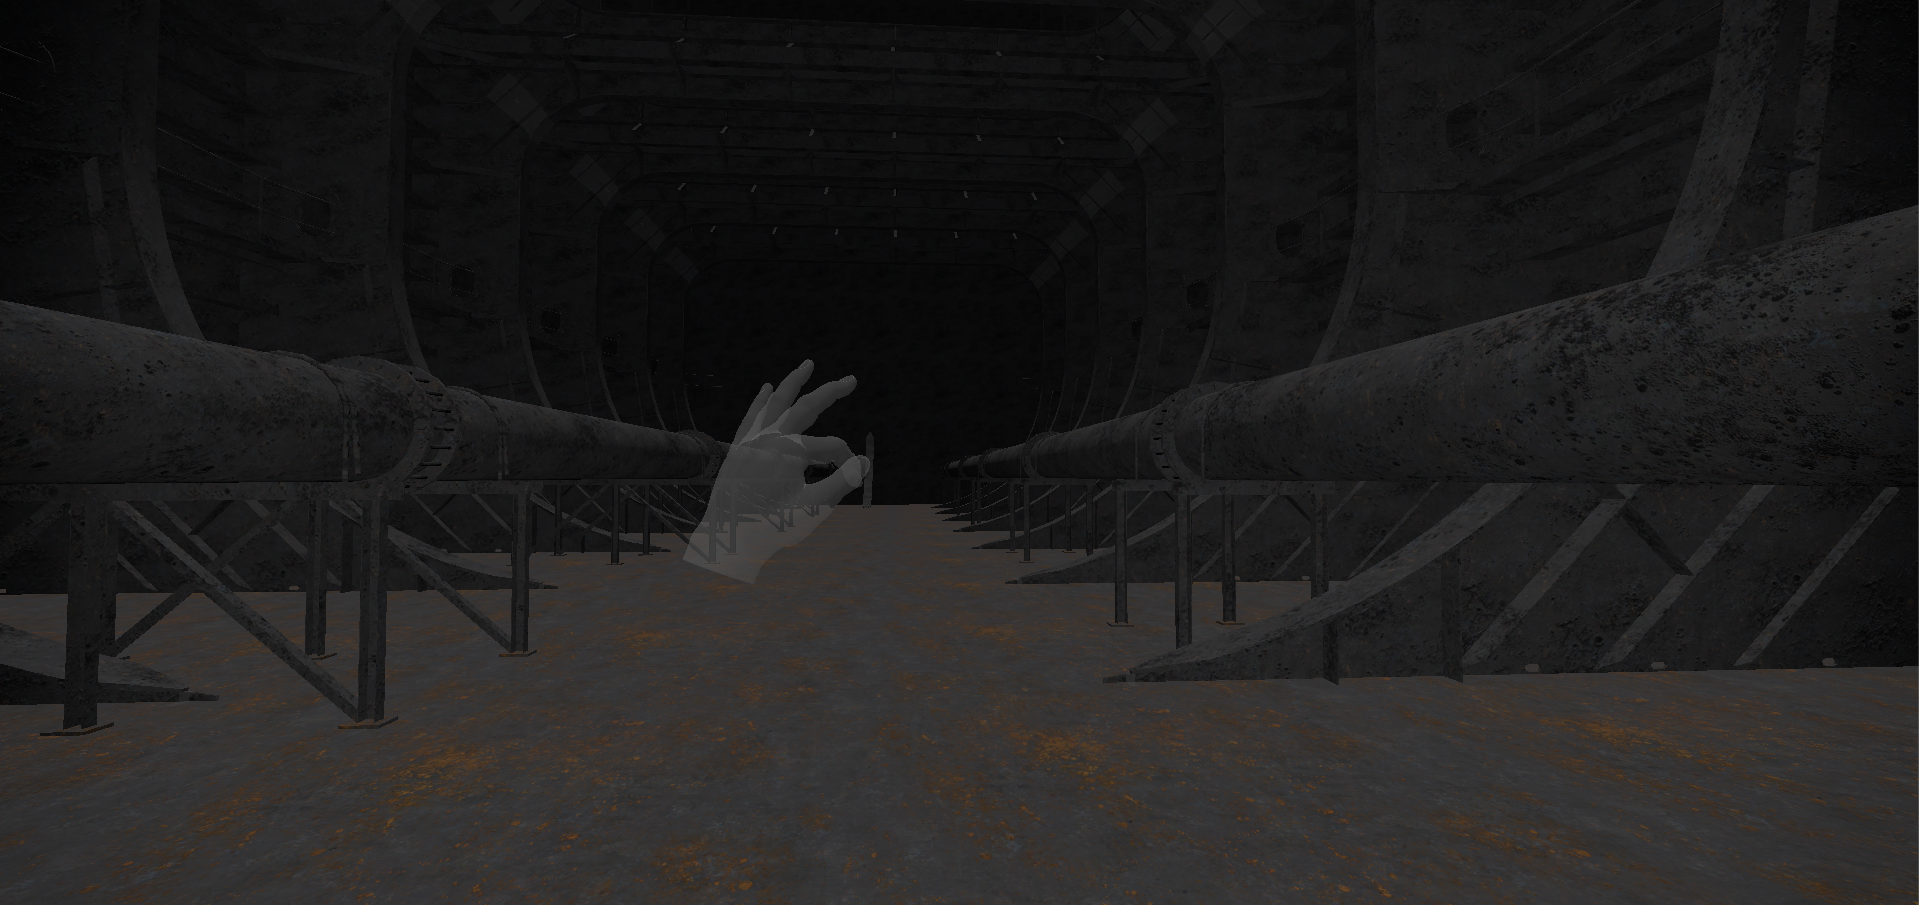
\includegraphics[width=\linewidth]{pictures/screenshots/gestures/disabled_detector.png}
	\caption[Disabled gestures]{When gestures are disabled, i.e all the detectors are disabled, the hand models are transparent}
	\label{fig:disabled_detector}
\end{figure} 

 
\section{The Detectors}
The detectors are represented as game objects and children of the \texttt{Detectors} game object under each hand game object. 
Each of these detector objects have the naming convention <gesture name> + "Detector" + <optional specifier> + "\_" + <handedness: Left or Right>, 
e.g.~\texttt{PinchDetectorStrict\_Left} and \texttt{FistDetector\_Right}. A certain detector of one hand is usual identical to the equivalent detector for the 
other hand with a few exception. These differences between hands are usually minor and will be mentioned when applicable. The detectors used in this implementation
utilizes a combination of several Leap Motion provided detectors, as these both cover the functional needs and are considered best practice. 
The Leap Motion provided detectors can as such be regarded as "base detectors", while the detectors that represents gestures in this implementation
can be regarded as "composite detectors". To differentiate between these two categories, the base detectors will be written in \textit{italic} or plain text, while
the composite detectors and game objects will be written in \texttt{monospace}.
The Leap Motion provided detectors utilized in the implementation is \textit{DetectorLogicGate}, \textit{PinchDetector}, \textit{ExtendedFingerDetector}, 
\textit{PalmDirectionDetector} and \textit{FingerDirectionDetector}.

The Leap motion base detectors provides some important parameters that can be set on a per detector instance basis, which often relates to thresholds values (e.g.~on/off values) and discrete
values (e.g~extended or not extended). Finding the optimal values for a certain gesture can often be the subject of a lot of adjustment and tweaking, as vision-based gesture recognition
technology often or always will be someone unprecice compared to e.g.~mouse and keyboard. The challenge is thus to find values that give a high amout of true positives (e.g.~the user attemps a gesture
and the gesture was recognized) and a low amount of false positives (e.g.~the user did not attempt a gesture and a gesture was recognized). 
During the implementation phase these values were adjusted several times in pursuit of the optimal values, and during the evaluation phase this was a much discussed topic were users often 
has their own "gesture sensitivity preferences" (this will be review in the next chapter). 

As was mentioned in the design, giving the user visual feedback when a gesture is recognized (i.e a detector is active) is probably a good idea.
In this implementation this is performed by changing the material of the hand models. The materials for each hand is listed in the handMaterials variable in the
\texttt{GestureHand} class, and follows the same order (or indecies) as the HandState enums specify (see \ref{tab:handstates}). 
Changing these materials is thus easy to do in Unity, but as default the following color-categories are used:
\begin{itemize}
\item Plain gold   - Used for gestures that perform rotations (only the pinch gesture).
\item Black 	   - Used for gestures that perform movement. This includes the Palm-down gesture (either y-axis movement or xyz-axes movement), 
			  		 Palm-side gesutre (x-axis movement) and the fist gesture (z-axis movement).
\item Glowing teal - Used for gestures that perform annotation interaction, i.e either places or edits annotations.
					 This includes the single point-gesture and the double point-gesture.
\item White 	   - Used when no gesture is performed (but gestures are still enabled).
\item Transparent  - Used when gestures are disabled.					
\end{itemize}

First the gesture implementations will be reviewed. 


\subsection{The PinchDetectorStrict and PinchDetectorSlack}
\begin{figure}%[h!] %[H]
	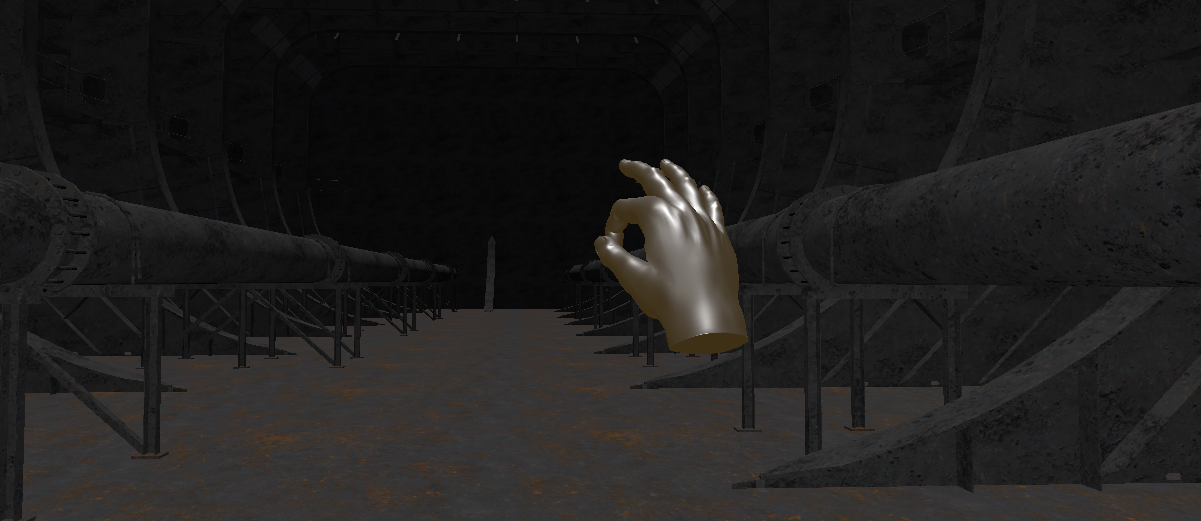
\includegraphics[width=\linewidth]{pictures/screenshots/gestures/pinch_detector2.png}
	\caption[The pinch gesture]{When the PinchDetector is active, i.e a pinch gesture is recognized, the hand is colored in a pale gold color.}
	\label{fig:pinch_detector2}
\end{figure} 

The \texttt{PinchDetectorStrict} and \texttt{PinchDetectorSlack} were originally one detector called \texttt{PinchDetector}, but was split up to represent two 
different options for the user. Both detectors utilize the base \textit{PinchDetector} script provided by the Leap Motion detection utilities, while the strict version
also uses the \textit{ExtendedFingerDetector}. The \texttt{PinchDetector} measures the distance between the tip of the thumb and index finger, and if these are below
a certain threshold (i.e the activate distance) the detector is active and signals \texttt{gestureCode}. If the distance grow larger than a set deactivate distance
the detector is deactivated. The activate distance used is 0.03 meter, while the deactivate distance is 0.06 meter. 

One problem with only having distance between the two finger tips as a criterion for the pinch gesture is that there would sometimes be false positives 
(i.e unintentional pinch gestures could occur). This was especially the case when attemping to perform the fist gesture as the distance between the tip of the
thumb and index finger is relatively small when the hand is a fist, and the application could thus sometimes perform a pinch gesture instead of a fist gesture.
Because of this the stricter version \texttt{PinchDetectorStrict} was created. This uses the same criterion as \texttt{PinchDetectorSlack}, but it also requires
that at least two fingers are extended. This is accompished by using the \textit{ExtendedFingerDetector} and \textit{DetectorLogicGate}. 
The finger states of the \textit{ExtendedFingerDetector} for all individual fingers are set to "either", meaning that, individually, each finger can 
be either extended or not extended, but on the "minimum extended" parameter 2 is set, while "maximum extended" is set to 5, 
meaning that anything between two and five fingers can be extended. 

\subsection{The PalmDownDetector}
\begin{figure}%[h!] %[H]
	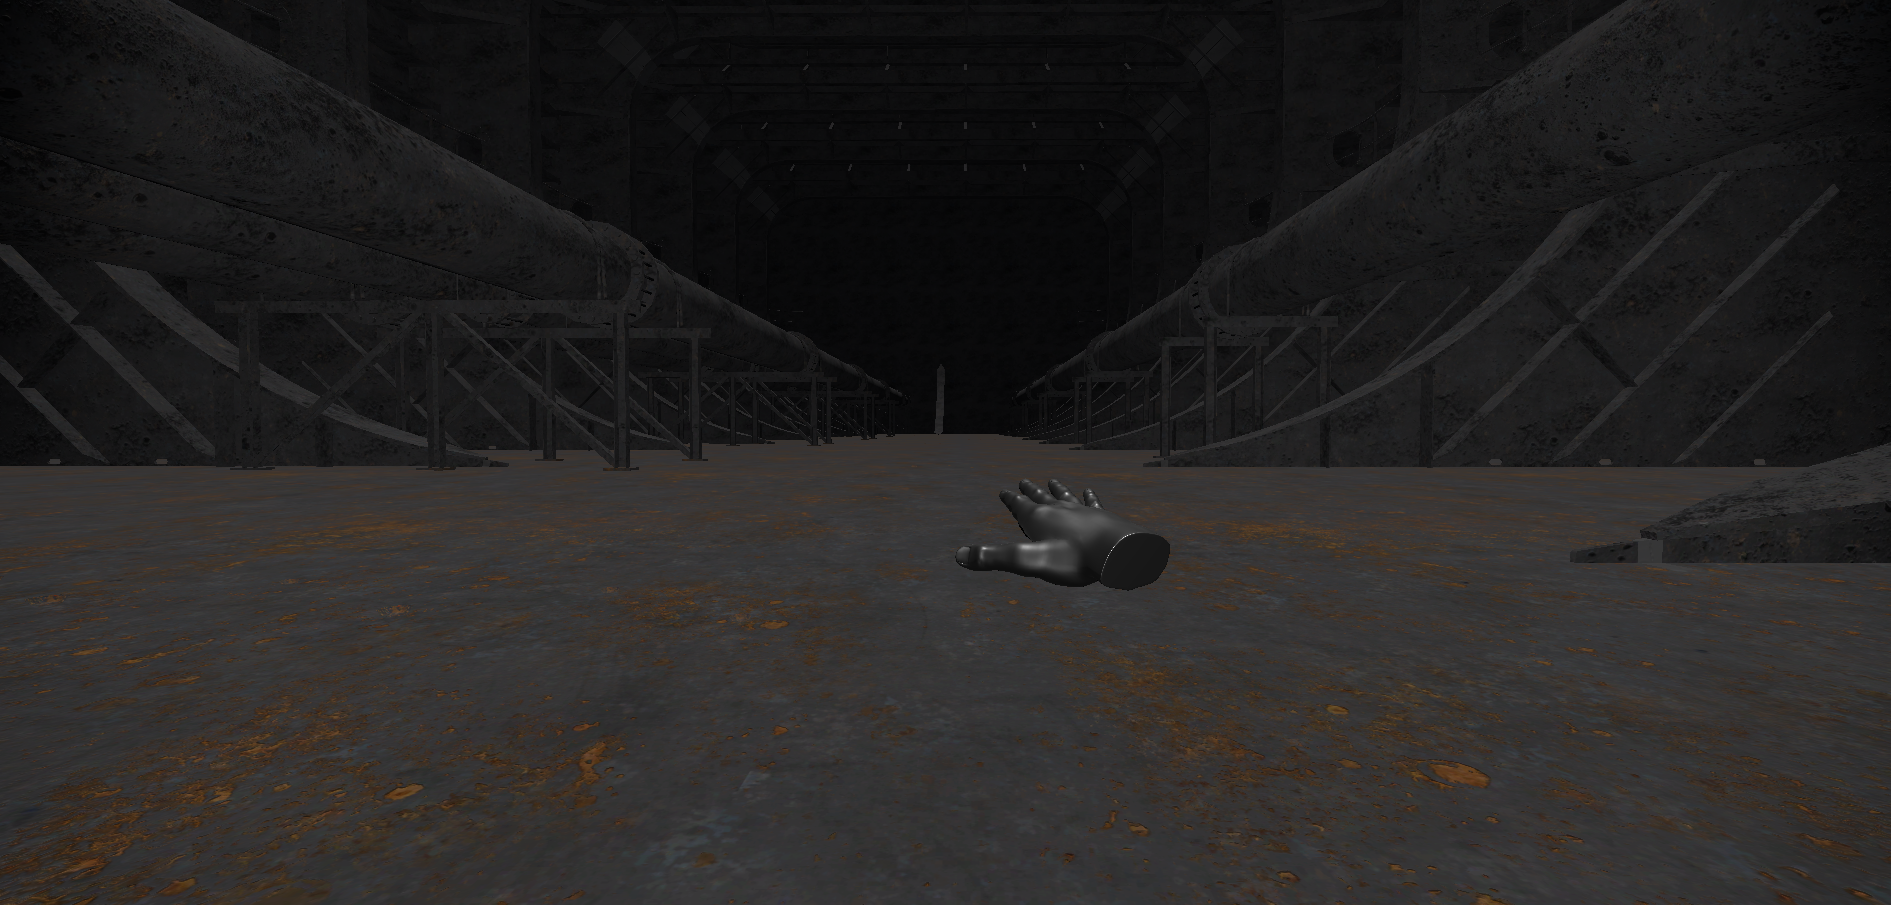
\includegraphics[width=\linewidth]{pictures/screenshots/gestures/palmdown_detector.png}
	\caption[The palmdown gesture]{When the PalmDownDetector is active, i.e a palm-down gesture is recognized, the hand is colored in a black.}
	\label{fig:palmdown_detector}
\end{figure}
The \texttt{PalmDownDetector} uses a PalmDirection detector and an ExtendedFinger detector, which is AND'ed by a DetectorLogicGate. 
The PalmDirectionDetector is configured to become active when the palm is pointing within 30 degrees of {0, -1, 0} (x = 0, y = -1, z = 0) direction, relative to the camera.
The coordinate system used functions just as if the three-dimensional axis had been drawn on the screen, so e.g.~ the coordinates {0, 0, 1} would be directly forward, while
{1, 0, 0} would be to the right.

The coordinates used for the PalmDirection Detector thus means that from the perspective of the camera, the palm should face directly downwords such that the 
palms are as parallell to the ground or table top.
The PalmDirectionDetector is also configured with an "On Angel" of 30 degrees and an "Off Angle" of 50. The detector is thus activated as long as the palm points within 
30 degrees of the desired direction, and is deactivated if the palm directions surpasses the threshold of 50 degree from the {0, -1, 0} direction.

The \texttt{PalmDownDetector} also used an ExtendedFingerdetector, as was covered in the previous section. This one is configured to require that 
the index-, middle, ring and pinky finger have to be extended, which the thumb can be either. 

\subsection{The PalmSideDetector}
\begin{figure}%[h!] %[H]
	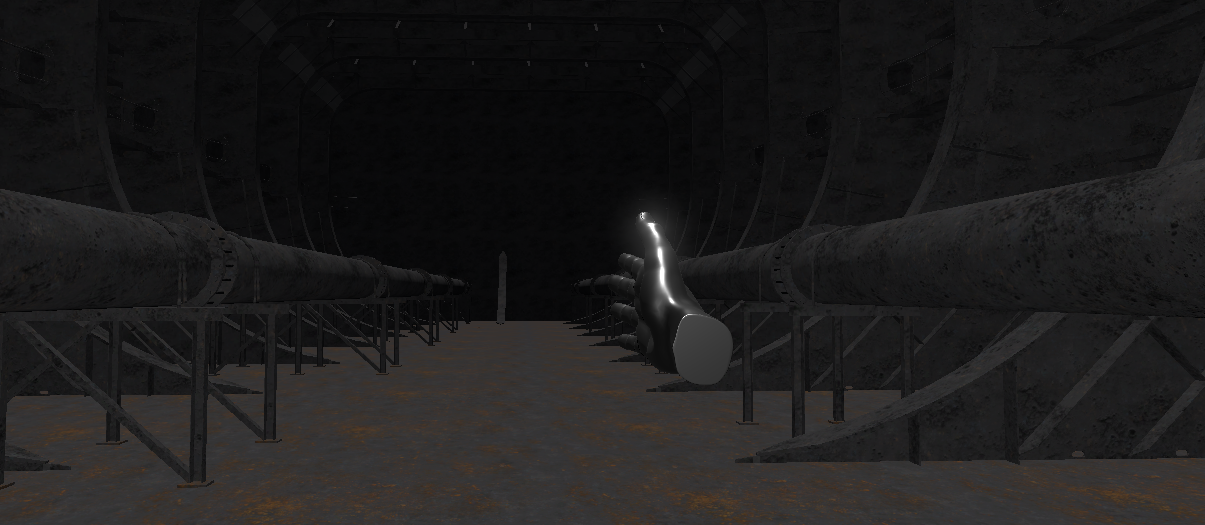
\includegraphics[width=\linewidth]{pictures/screenshots/gestures/palmside_detector.png}
	\caption[The palmside gesture]{When the PalmSideDetector is active, i.e a palm-side gesture is recognized, the hand is colored in a black.}
	\label{fig:palmside_detector}
\end{figure} 

The \texttt{PalmSideDetector} is quite similar to the \texttt{PalmDownDetector} and uses the same detectors, but with a different configuration. 
Although the settings used for the DetectorLogicGate and the ExtendedFingerDetector are very similar, the settings for the PalmDirectionDetector differs.
Unlike the \texttt{PalmDownDetector}, where both hands are required to point in the direction {0, -1, 0} to perform the gesture, the \texttt{PalmSideDetector} makes 
a distinction here. This is because requiring the palm direction {1, 0, 0} (right) is reasonable for the left hand, as it is within its natural range of motion, but
for the right hand this requires the whole arm to twist. The required palm direction for the left hand is thus {1, 0, 0} (right), and {-1, 0, 0} (left) for the right hand, both
with an "On Angel" of 30 degrees and an "Off Angle" of 50.

\subsection{The FistDetector}
\begin{figure}%[h!] %[H]
	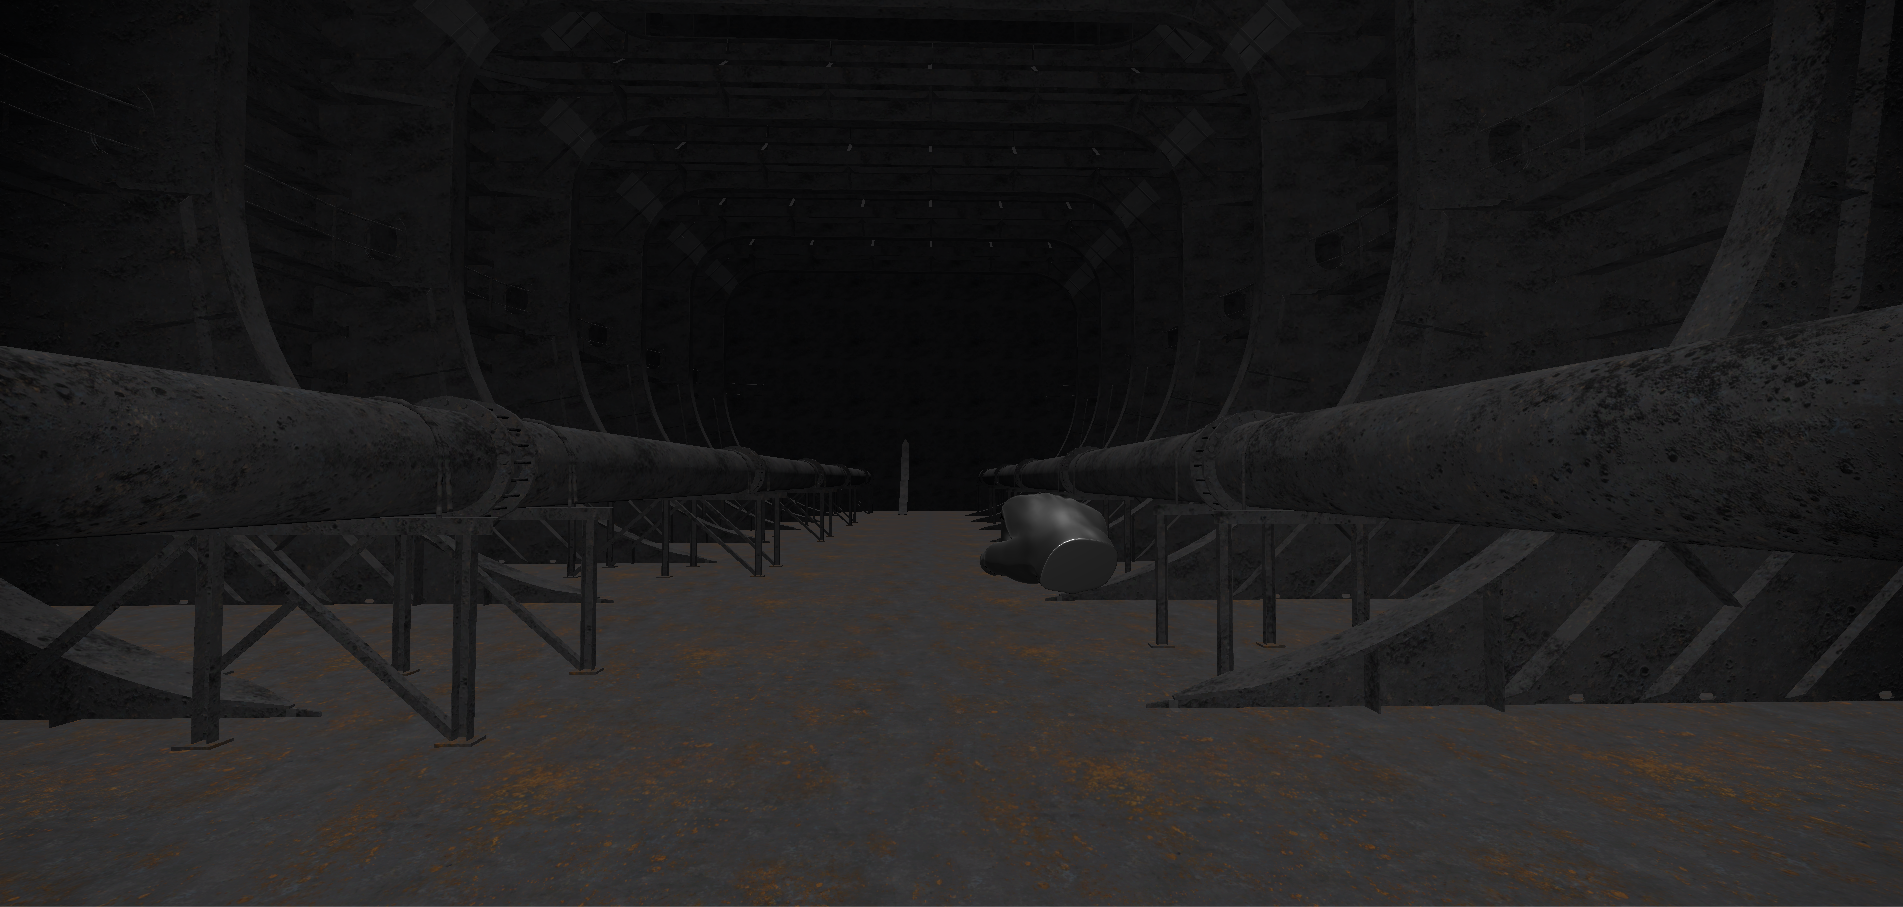
\includegraphics[width=\linewidth]{pictures/screenshots/gestures/fist_detector.png}
	\caption[The fist gesture]{When the FistDetector is active, i.e a fist gesture is recognized, the hand is colored in a black.}
	\label{fig:fist_detector}
\end{figure} 
The \texttt{FistDetector} is prehaps the simplest of the detectors and only uses the ExtendedFingerDetector.
The ExtendedFingerDetector is simply configured to require that no finger is extended. 
As such the minimum- and maximum amount of fingers extended are both set to 0, and all finger have their required state set to "Not Extended"

\subsection{The SinglePointDetector}
\begin{figure}%[h!] %[H]
	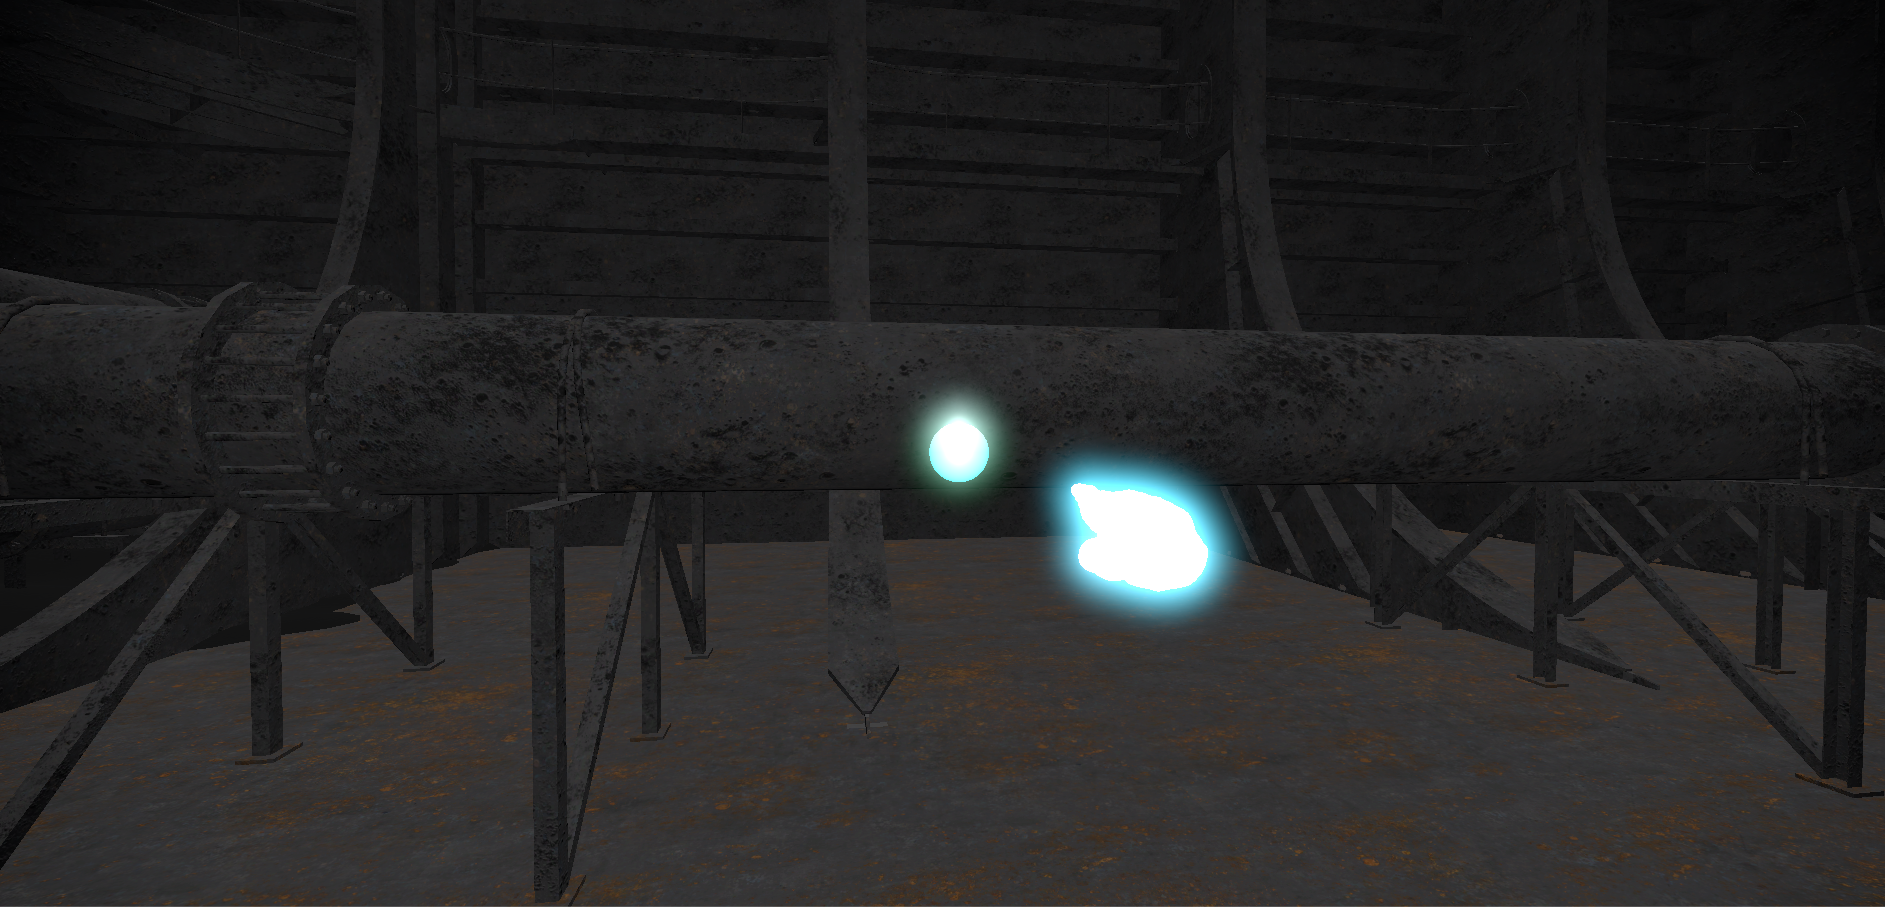
\includegraphics[width=\linewidth]{pictures/screenshots/gestures/singlepoint_detector.png}
	\caption[The single-point gesture]{When the SinglePointDetector is active, i.e a single-point gesture is recognized, the hand is colored in a glowing teal color.}
	\label{fig:singlepoint_detector}
\end{figure} 
The \texttt{SinglePointDetector} uses two detectors, ExtendedFingerDetector and FingerDirectionDetector, bound together with an AND-DetectorLogicGate.
The ExtendedFingerDetector here requires that the index finger is extended and that the middle-, ring- and pinky fingers are not extended (both thumb states are accepted).
The FingerDirectionDetector is set to be active when the index finger points within 15 degrees of the direction {0, 0, 1}, relative to the camera.
Both the "On Angle" and "Off Angle" settings are set to 15 in this detector, as, unlike the previously mentioned detectors, this one is not of a "continous nature".
Simply put, the previous gestures can last as long as the gesture is held, and while this is the case the application continously watches the active hands and responds to
hand movements. The single- and double point detectors are techniqually also continous and can last as long as the user desires, 
but as soon as these gestures are activated their discrete action is performed. After this action has been performed no other action will be performed by the same
and while the same gesture is kept. In the case of both the single- and double point detectors, an annotation is either placed or edited upon activation. 
If a user thus with to place an annotation and immediatly edit it, he or she has to use the approprate gesture, release the gesture and do the same gesture again.

\subsection{The DoublePointDetector}
\begin{figure}%[h!] %[H]
	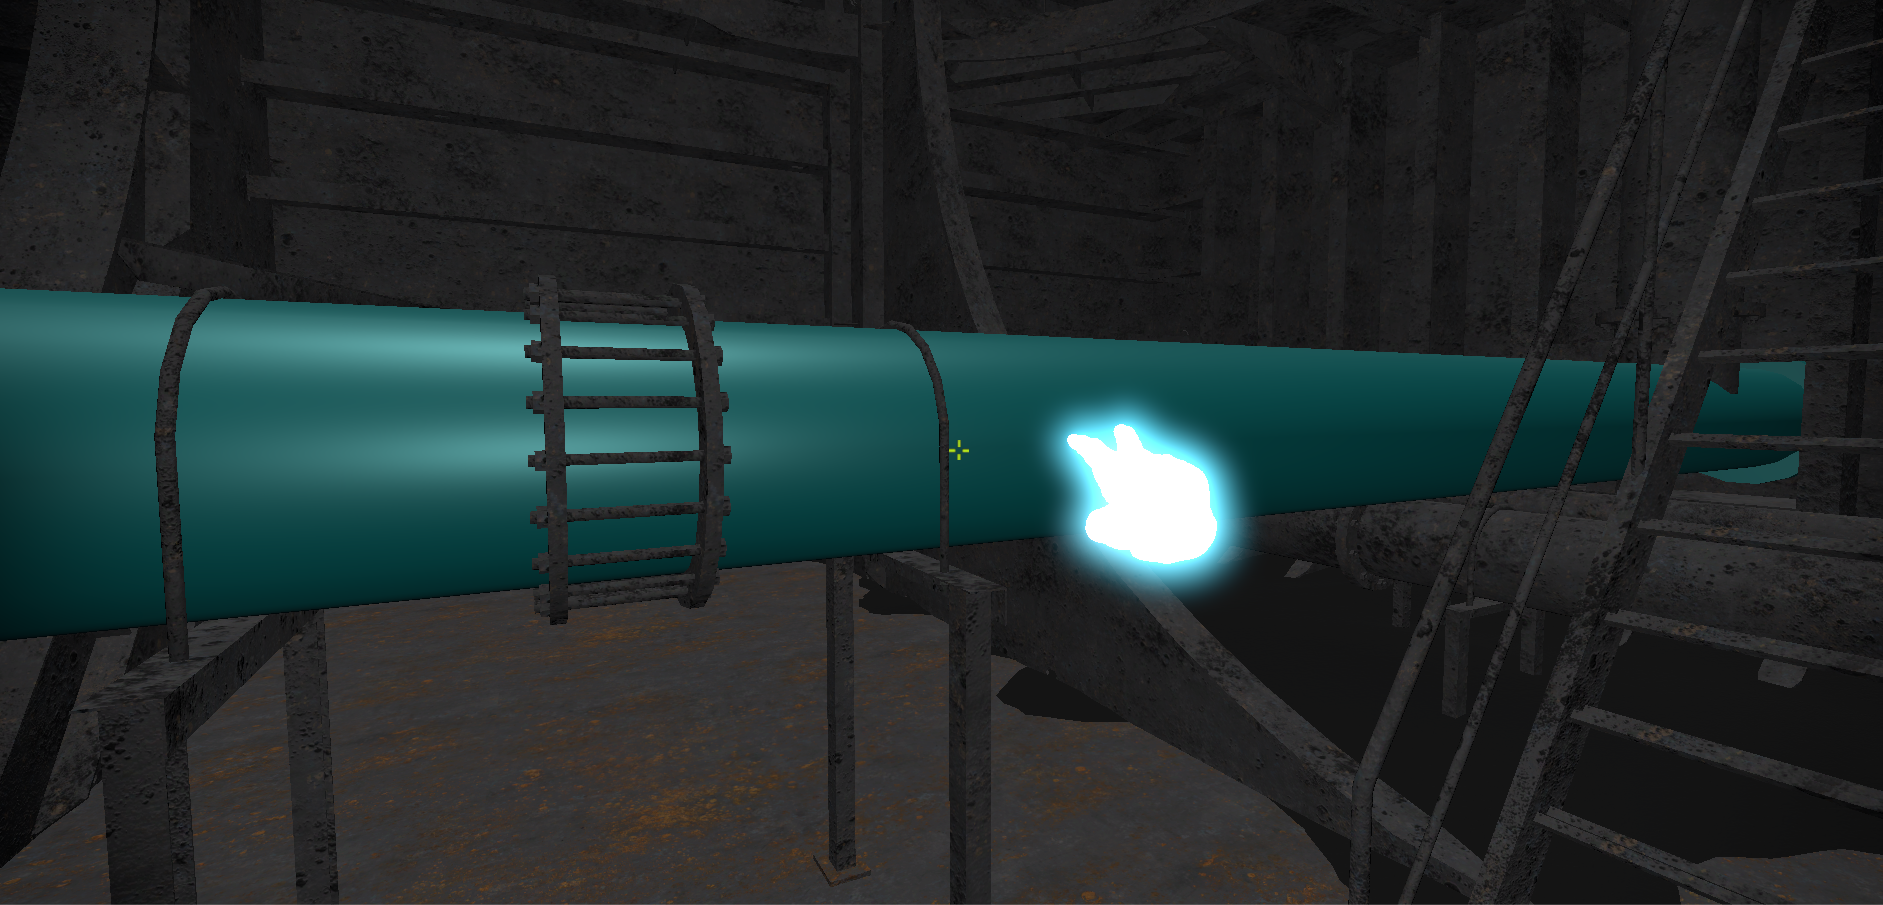
\includegraphics[width=\linewidth]{pictures/screenshots/gestures/doublepoint_detector.png}
	\caption[The double-point gesture]{When the DoublePointDetector is active, i.e a double-point gesture is recognized, the hand is colored in a glowing teal color.}
	\label{fig:doublepoint_detector}
\end{figure} 
The \texttt{DoublePointDetector} is similar to the \texttt{SinglePointDetector} and uses the same base detectors. 
The only implementational difference between this two is that the ExtendedFingerDetector is configured to require that both the index- and middle finger are extended, while
the ring- and pinky finger are contracted (both thumb states are accepted).


% Write about the menu?
\section{The Menu}
The menu is opened when the palm of the left hand is facing towards the camera, and can be interacted with using the index finger of the right hand.
Unlike the other gestures-enabled commands the menu is implemented through the use of the open source project Hover UI Kit, created by Aesthetic Interactive~\citep{Hoverkit}.
The Hover UI Kit project offer three different interface modules: Hovercast, Hoverkey and Hoverpanel, where Hovercast is the one the menu is based on.
This means that several of the menu's interaction components, such as registering button clicks are handled by the Hover UI kit package.

\begin{figure}%[h!] %[H]
	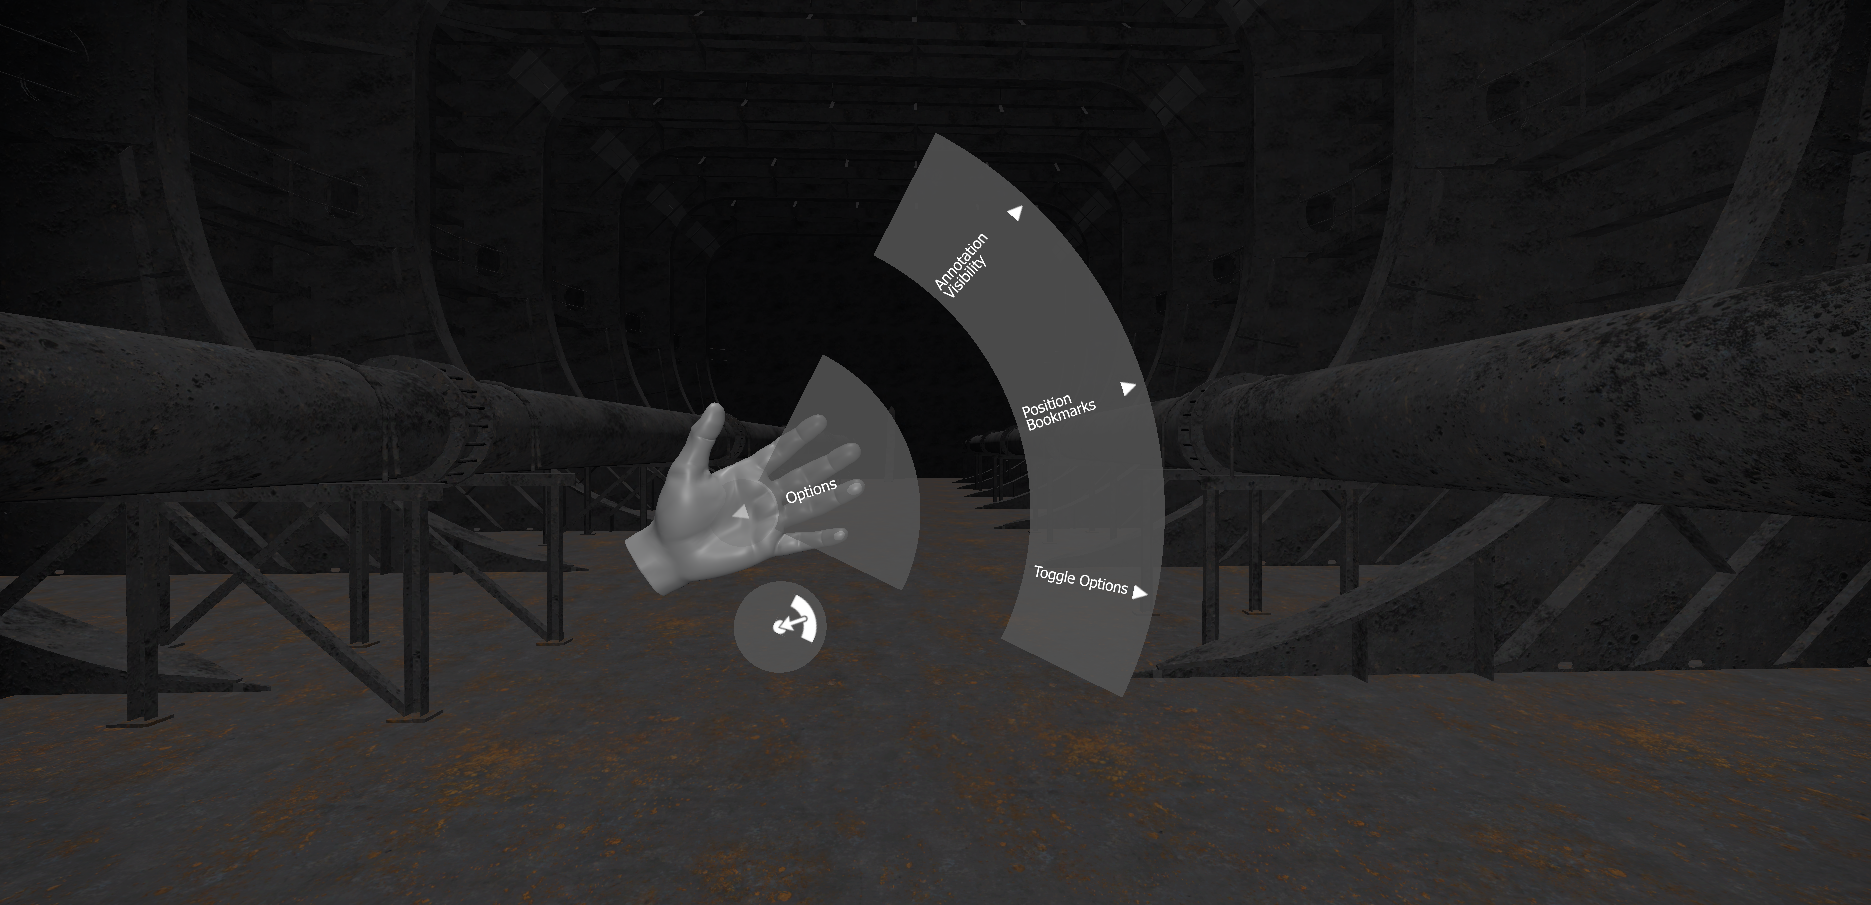
\includegraphics[width=\linewidth]{pictures/screenshots/gestures/menu_detector.png}
	\caption[The Menu]{The menu is opened when the palm of the left hand is facing towards the camera, and can be interacted with using the index finger of the right hand.}
	\label{fig:menu_detector}
\end{figure} 

The Hover UI kit main game object is present in the \texttt{GestureMenu} game object, which is a top-level game object in the project hierarchy.
\texttt{GestureMenu} has four child game object: \texttt{Hovercast}, \texttt{CursorRenderer} (which is disabled by default), \texttt{MenuHandler} and \texttt{Hoverkit}.
\texttt{Hovercast} represent the menu itself and contains the hierarchy of game objects that represents the menu buttons. 
\texttt{CursorRenderer} can optionally render a ring/cursor around the fingers that can be used as cursors.
By default only the index finger of the right hand can be used to select elements in the menu.
\texttt{MenuHandler} contains the scripts \texttt{ToggleOptions}, \texttt{Bookmarks} and \texttt{AnnotationVisibility}, which are all responsible for handling
the different actions accessable from the menu.
Lastly, the \texttt{Hoverkit} game objects contains some important "management scripts" (e.g.~\texttt{HoverItemsManager} and \texttt{HoverInteractionSettings}) related to the 
different functionality of the Hovercast menu and hoverkey keyboard in the annotation form (more on that later). The \texttt{Hoverkit} game object also
contains a Cursor game object, which contains a hierarchy with representations of the left- and right hand, and then each hand's respective finger objects. 
In this object hierarchy we can select which fingers that are cursors, which hand that can "host" or "spawn" the menu etc. As mentioned earlier
the default setting is that the menu only can be created by the left hand palm and only interacted with using the right hand index finger. 
 
\subsection{The Menu Objects}
The \texttt{Hovercast} game object has four game objects as direct children, which all represent a visible part of the hovercast menu:
\texttt{OpenItem}, \texttt{TitleItem}, \texttt{BackItem} and \texttt{Rows}. 

\begin{figure}%[h!] %[H]
	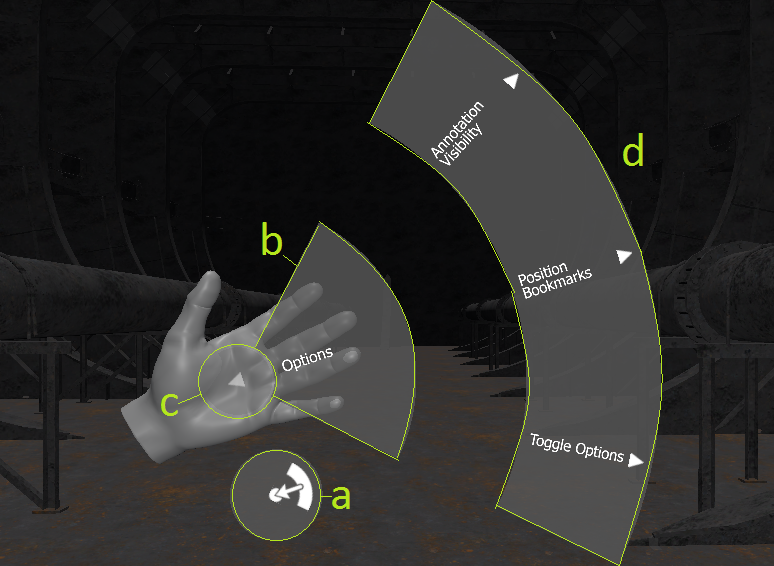
\includegraphics[width=\linewidth]{pictures/screenshots/menu/menu_components.png}
	\caption[The Menu components]{The main menu object is represented with four sub-objects: \texttt{OpenItem} (a), \texttt{TitleItem} (b), \texttt{BackItem} (c) 
			 and \texttt{Rows} (d).}
	\label{fig:menu_components}
\end{figure}

While the \texttt{OpenItem}, \texttt{TitleItem} and \texttt{BackItem} uses functionality that is the default in Hover UI Kit, and is readily available in presets,
\texttt{Rows} contains quite a bit of implementation specific objects. The term "row" will her refer to a set of one or more buttons, which are clickable and visible at together,
in the "row section" of the menu (see \ref{fig:menu_components} (d)). The \texttt{Rows} game object has four direct children: \texttt{Root}, \texttt{RowA}, \texttt{RowB} 
and \texttt{RowC}. \texttt{Root} is the root menu row, i.e the row that is visible when the menu is opened, and contains three buttons, each represented as 
child game objects of \texttt{Root}: \texttt{ItemA}, \texttt{ItemB} and \texttt{ItemC}. Each of these buttons leads to their own submenu, i.e their own row. 
\texttt{ItemA} represent the "Annotation Visibility" submenu, and brings up \texttt{RowA} as the "current row" instead of root when clicked. \texttt{ItemB} ("Position Bookmarks") 
and \texttt{ItemC} ("Toggle Options") follows the same logic and lead to \texttt{RowB} and \texttt{RowC} respectively (see \ref{table:menu_hierarchy} for the hierarchical overview. 
This transition is handled by the \texttt{HovercastRowSwitchingInfo} component that is attached to each button game object.  

\renewcommand{\DTstyle}{\textrm\expandafter\raisebox{-0.7ex}}
\DTsetlength{1em}{1em}{0.2em}{0.4pt}{0.4pt}
\setlength{\DTbaselineskip}{2\baselineskip}

\begin{table}[]
\label{table:menu_hierarchy}
	\dirtree{%
	.1 Root menu.
	.2 Annotation Visibility (submenu/row).
	.3 Always visible (radio button).
	.3 Visible with LOS (radio button).
	.3 Invisible (radio button).
	.3 Use Glow (checkbox).
	.3 Back (button).
	.2 Position Bookmarks (submenu/row).
	.3 Origin (button).
	.3 Back (button).
	.2 Toggle Options (submenu/row).
	.3 Toggle crosshair (button).
	.3 Enable gestures/Disable gestures (button).
	.3 Combined XYZ gestures/Distinguish XYZ gestures (button).
	.3 Back (button).
	}
\caption[The Menu Hierarchy]{The Menu Hierarchy}
\end{table}

\texttt{RowA}, \texttt{RowB} and \texttt{RowC} each contains game objects that represents buttons in that submenu. 
In these button game objects \texttt{HoverItemDataSelector}, \texttt{HoverItemDataRadio} or \texttt{HoverItemDataCheckbox}, for "regular buttons", radio buttons and 
checkboxes respectively, are attached as components. These components are all either directly or indirectly subclasses of \texttt{HoverItemDataSelectable}, which 
contains important properties like "Label" (i.e the button text value) and a list of eventhandler. An example of this is \texttt{ItemCB} in \texttt{RowC}, which has 
the label "Disable Gestures" and has an entry in the "OnSelectedEvent" list. This entry is a reference to the \texttt{GestureOptions} class' function \texttt{toggleGestures}. 

\subsection{The MenuHandler Scripts}
The menu makes use of three scripts to handle all actions: \texttt{AnnotationVisibility}, \texttt{Bookmarks} and \texttt{GestureOptions}.
These are all components of the \texttt{MenuHandler} game object and serve their seperate submenus (i.e Row A, B and C) and buttons. 

The \texttt{AnnotationVisibility} script's main purpose is to interact with the active camera rig's annotation camera, and manipulate the way
the annotations are presented to the user. This include choosing between three annotation presentation modes: "Always visible", "Visible with LOS" and 
"Invisible", and choosing whether to use a glow effect on annotation or not. This is done by manipulating the active annotation camera's culling mask 
and clear flags using bit shift:

\begin{table}
\label{table:annotation_visibility_code}
\lstset{style=csharp}
\begin{lstlisting}
public void alwaysShow()
{
	//to toggle a bit on and off, use XOR
	annotationCamera.cullingMask |= 1 << LayerMask.NameToLayer("SphereAnnotation");
	annotationCamera.clearFlags = CameraClearFlags.Depth;
}

public void showWithLOS()
{
	annotationCamera.cullingMask |= 1 << LayerMask.NameToLayer("SphereAnnotation");
	annotationCamera.clearFlags = CameraClearFlags.Nothing;
}

public void hide()
{
	// Only render objects in the first layer (Default layer)
	annotationCamera.cullingMask &= ~(1 << LayerMask.NameToLayer("SphereAnnotation"));
}
\end{lstlisting}
\caption[Annotation visibility manipulation]{Annotation visibility manipulation example in C\# code. This code snippets makes use of 
		bit shifts on the annotation camera's culling mask and clear-flags properties.} 
\end{table}

The functional differences between the annotation presentation mode with or without glow are covered in \ref{sec:annotations}. 

The \texttt{Bookmarks} script's main purpose is to handle what in the menu is refered to as "Positional bookmarks". The primary idea behind positional bookmarks 
is to allow the user to save specific points of interest in the model to be able to quickly return there, just like one could bookmark a web page in a web browser. 
In the current iteration of the application it isn't possible to create new bookmarks, so the only available one is the "Origin" bookmark, which is the position and orientation
the user has when first entering the application (useful to reset the position e.g.~ if the user should get lost in some way). In the script this functionality is accomplished
by having a linked list of transforms (a unity game object component storing relevant information) and a referance to the \texttt{MasterController} game object. 
The \texttt{MasterController}'s position and rotation in the applications first rendered frame is stored as the first entry in this list and, should the user click the 
appropriate menu button "Origin", in the "Positional bookmarks" submenu, the function \texttt{GoToBookmark(int index)} should be called with index = 0 as index argument. 
The \texttt{GoToBookmark} function then looks up the transform stored at index \textit{i}, and if successful sets the position and orientation coordinates of the 
\texttt{MasterController}'s transform. The user will experience this as the camera "teleporting" to the same spot as the player started on when entering the 3D model.

The \texttt{GestureOptions} script's main purpose is to handle options related to gestures, and handles two menu elements from the Toggle Options submenu:
"Enable gestures" / "Disable gestures" (one button with a context dependent label) and "Combine XYZ gestures" / "Distingush XYZ gestures" (also context dependent label). This is 
primarily done by two of its functions \texttt{toggleGesturesActive} and \texttt{toggleGestureMode}, which both use the context dependent toggle principle 
and functions in the \texttt{GestureHand} class. In the implementation a toggle is simply to swap to the opposite value of the current, with two possible values available (i.e 
toggle + true = false and toggle + false = true).


\texttt{toggleGesturesActive} checks the value of the instance variable \texttt{GesturesEnabled} 
and either disables or enables gestures based on what is variable holds. If \texttt{GesturesEnabled = true}, i.e that gestures are enabled, the function 
disables gestures by calling each \texttt{GestureHand}'s \texttt{disableDetectors} function, swaps hand materials to the "disabled-material" and swaps the 
\texttt{GesturesEnabled} variable to its opposite value (i.e now \texttt{GesturesEnabled = false}). In the opposite case, i.e when the function is called and 
the \texttt{GesturesEnabled} variable has the value false, gestures are enabled by calling each \texttt{GestureHand}'s \texttt{enableDetectors} function, swapping
hand materials to the "none-material" and swapping the \texttt{GesturesEnabled} variable to its opposite value (i.e now \texttt{GesturesEnabled = true}). 

\begin{table}
\label{table:gesture_options_code}
\lstset{style=csharp}
\begin{lstlisting}
public GestureHand[] hands;
private static bool gesturesEnabled;

public void toggleGesturesActive(HoverItemDataSelector selector)
{
	if (gesturesEnabled)
	{
		selector.Label = "Enable Gestures";
		foreach (GestureHand hand in hands)
		{
			hand.disableDetectors();
			hand.ToggleHandMaterial(hand.handMaterials[7]);
		}

	}
	else
	{
		selector.Label = "Disable Gestures";
		foreach (GestureHand hand in hands)
		{
			hand.enableDetectors();
			hand.ToggleHandMaterial(hand.handMaterials[0]);
		}
	}

	gesturesEnabled = !gesturesEnabled;
}
\end{lstlisting}
\caption[The GestureOptions class]{The GestureOptions class can be called to enable or disable all detectors based on its current state.} 
\end{table}

The \texttt{toggleGestureMode} functions in a very similar manner as \texttt{toggleGesturesActive} and uses a boolean value present in the \texttt{GestureHand} instances
to toggle between a combined or separate state for movement gesture (i.e whether to have movement gestures in the x, y and z plans combined or separate.   

\section{The Annotations}


%About how annotations are implemented

\subsection{Annotation Visibility Levels}
\label{sec:annotations}
Annotation visibiliy levels can be access through the menu and decides how annotations appear the the virtual world. 

\begin{figure}%[h!] %[H]
	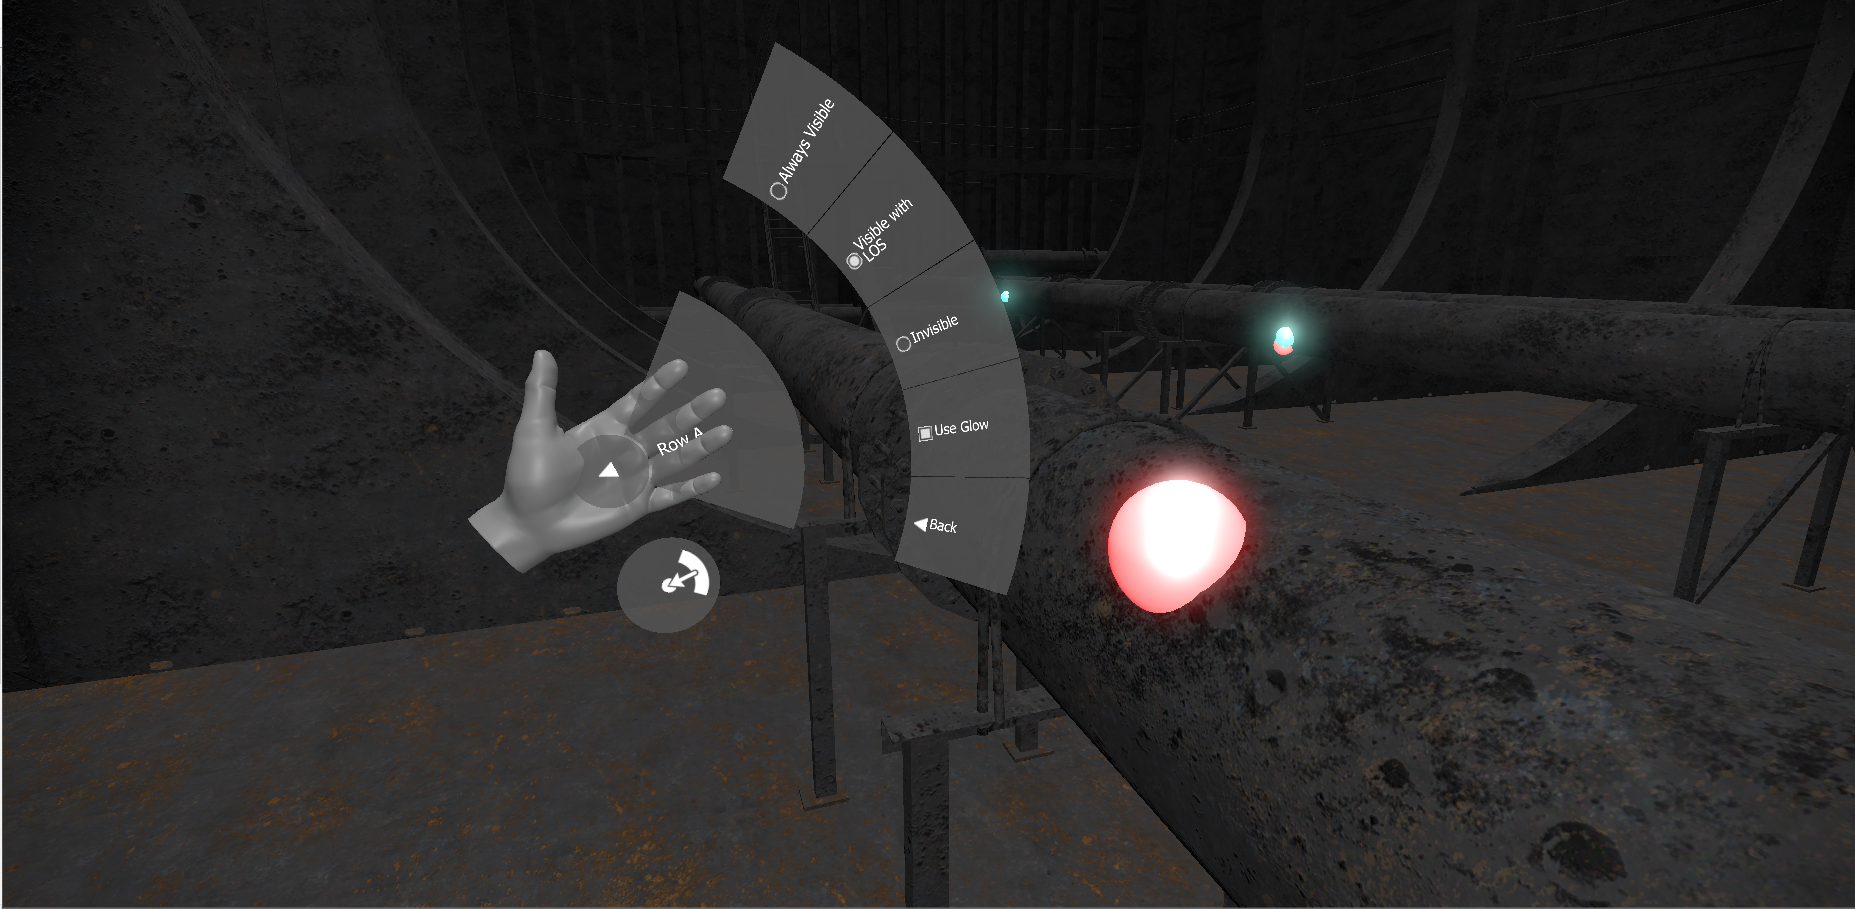
\includegraphics[width=\linewidth]{pictures/screenshots/annotation_visibility/annotation_visibility_options.png}
	\caption[The Annotation Visibility Submenu]{The user can decide three different annotation visibility settings in the Annotation Visibility Submenu.}
	\label{fig:annotation_visibility_options}
\end{figure} 

\begin{figure}%[h!] %[H]
	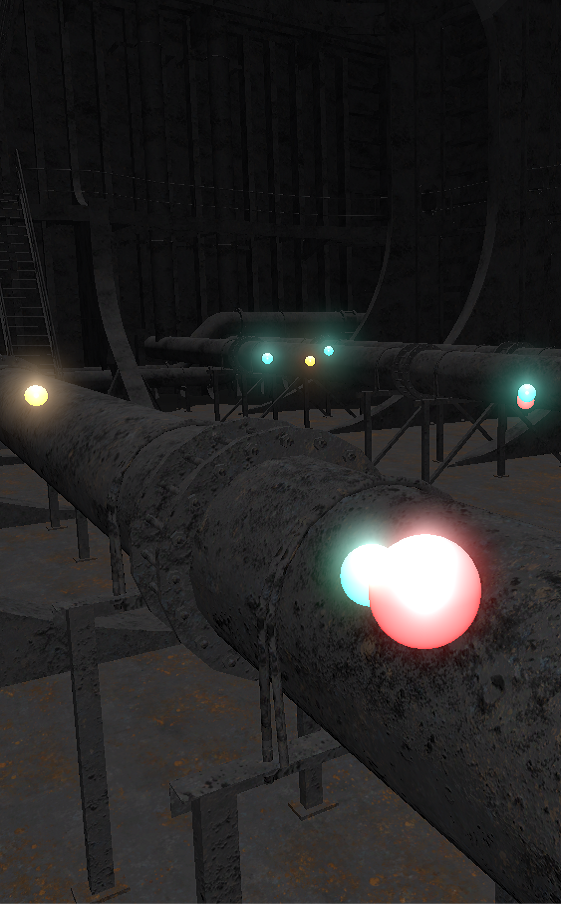
\includegraphics[width=0.32\linewidth]{pictures/screenshots/annotation_visibility/side_by_side/always_visible_small.png}
	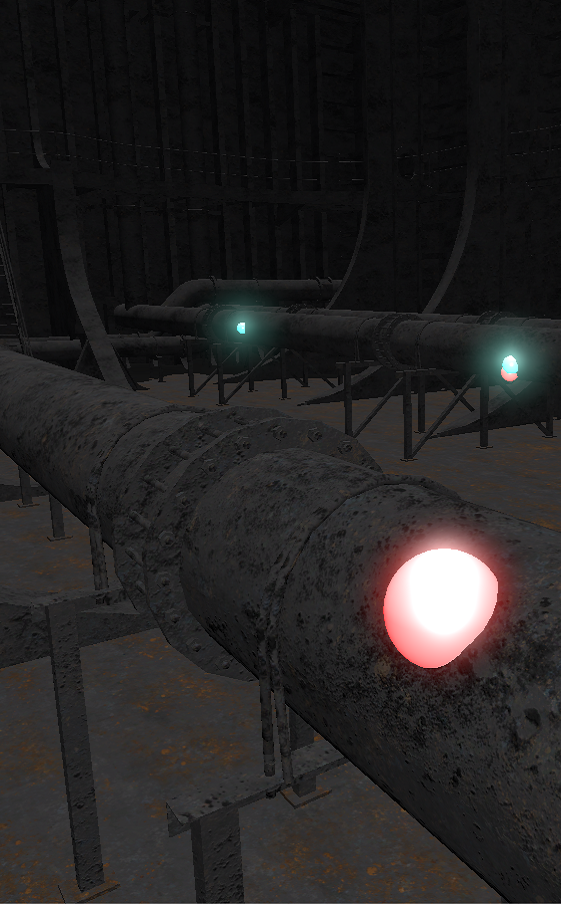
\includegraphics[width=0.32\linewidth]{pictures/screenshots/annotation_visibility/side_by_side/LOS_visible_small.png}
	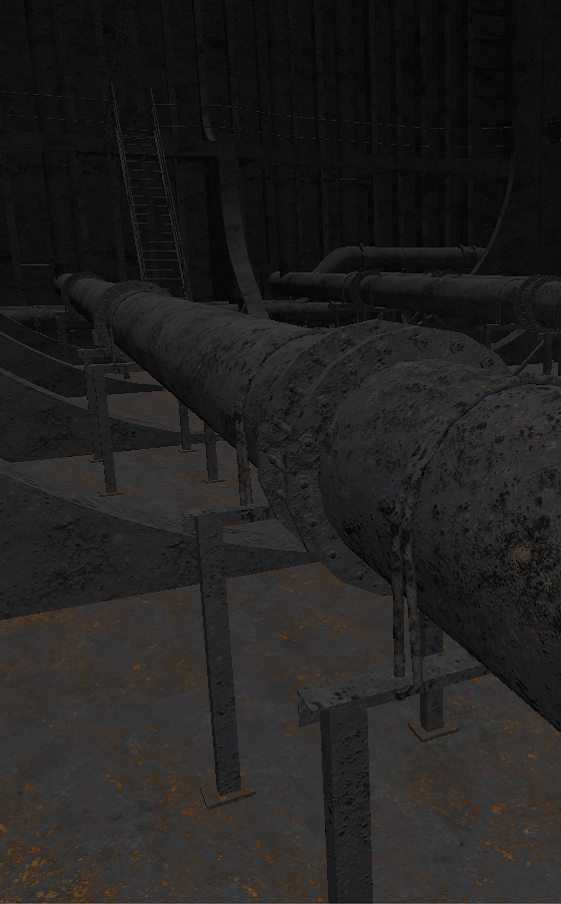
\includegraphics[width=0.32\linewidth]{pictures/screenshots/annotation_visibility/side_by_side/invisible_small.png}
	\caption[Annotation visibility levels comparison]{A side-by-side comparison of the annotation visibility levels. These three pictures are taken with the same camera position
	and orientation using different visibility settings. When selecting the "Always visible" option (left picture) annotations are not occluded and thus always visible, even through other objects like
	the pipes present in this picture. When selecting the "Visible with LOS" option (middle picture) annotations are only visible with line of sight. 
	If the user selects the "Invisible" option (right picture) are not visible and can not be interacted with.}
	\label{fig:visibility_comparison}
\end{figure} 



\paragraph{Visible with Line Of Sight}
% \begin{figure}%[h!] %[H]
% 	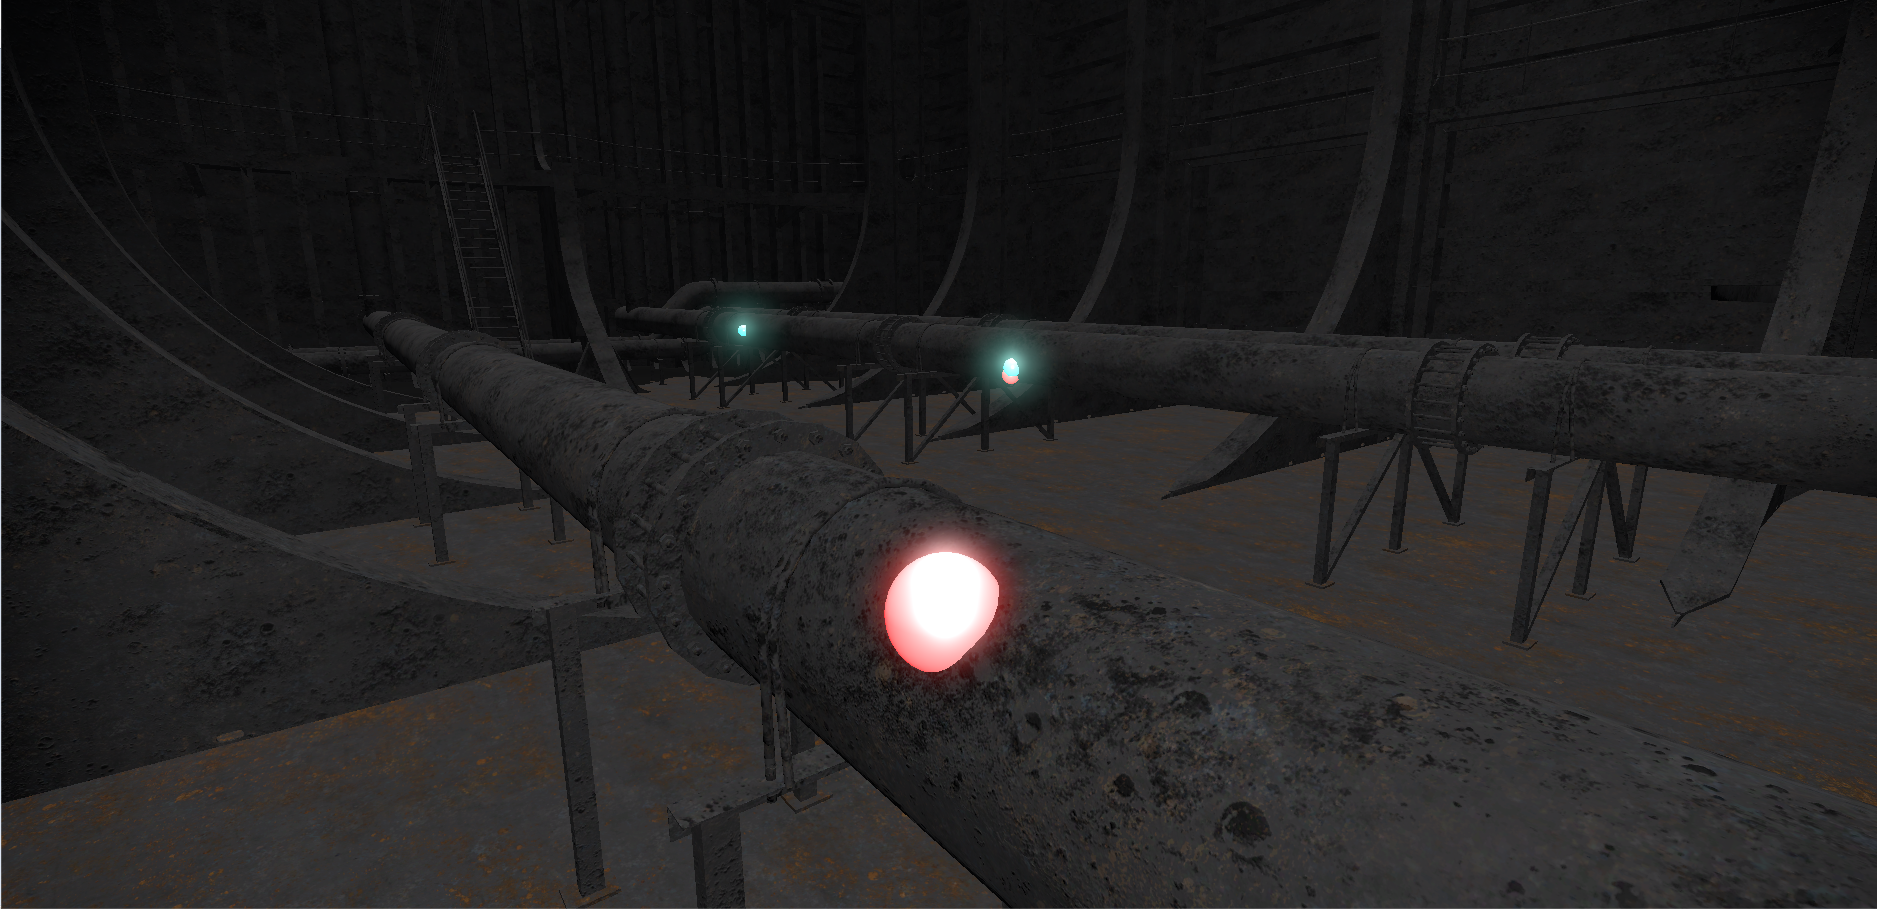
\includegraphics[width=\linewidth]{pictures/screenshots/annotation_visibility/LOS_visible.png}
% 	\caption[Annotations only visible with LOS]{When selecting the "Visible with LOS" option in the Annotation Visibility Submenu annotations are only visible with 
% 				line of sight.}
% 	\label{fig:LOS_visible}
% \end{figure} 


\paragraph{Always Visible}
\begin{figure}%[h!] %[H]
	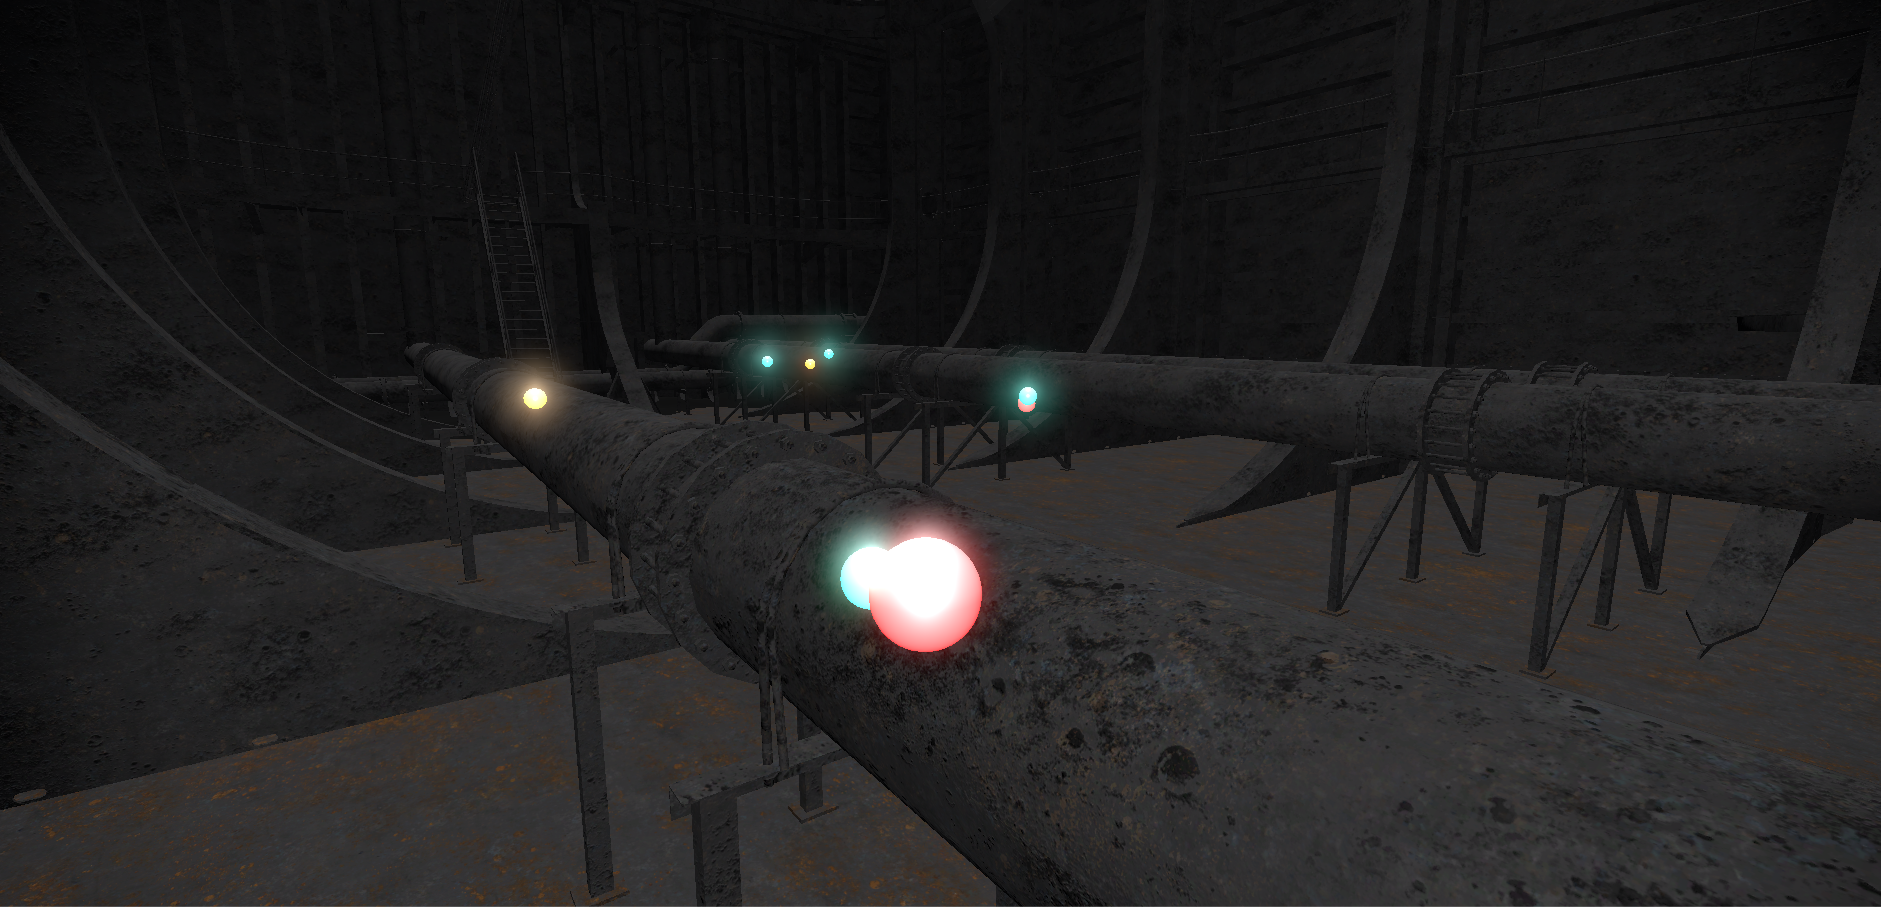
\includegraphics[width=\linewidth]{pictures/screenshots/annotation_visibility/always_visible.png}
	\caption[Annotation always visible]{When selecting the "Always visible" option in the Annotation Visibility Submenu annotations are not occluded and thus always visible, 
	even through other objects.}
	\label{fig:always_visible}
\end{figure} 

\paragraph{Invisible}
% \begin{figure}%[h!] %[H]
% 	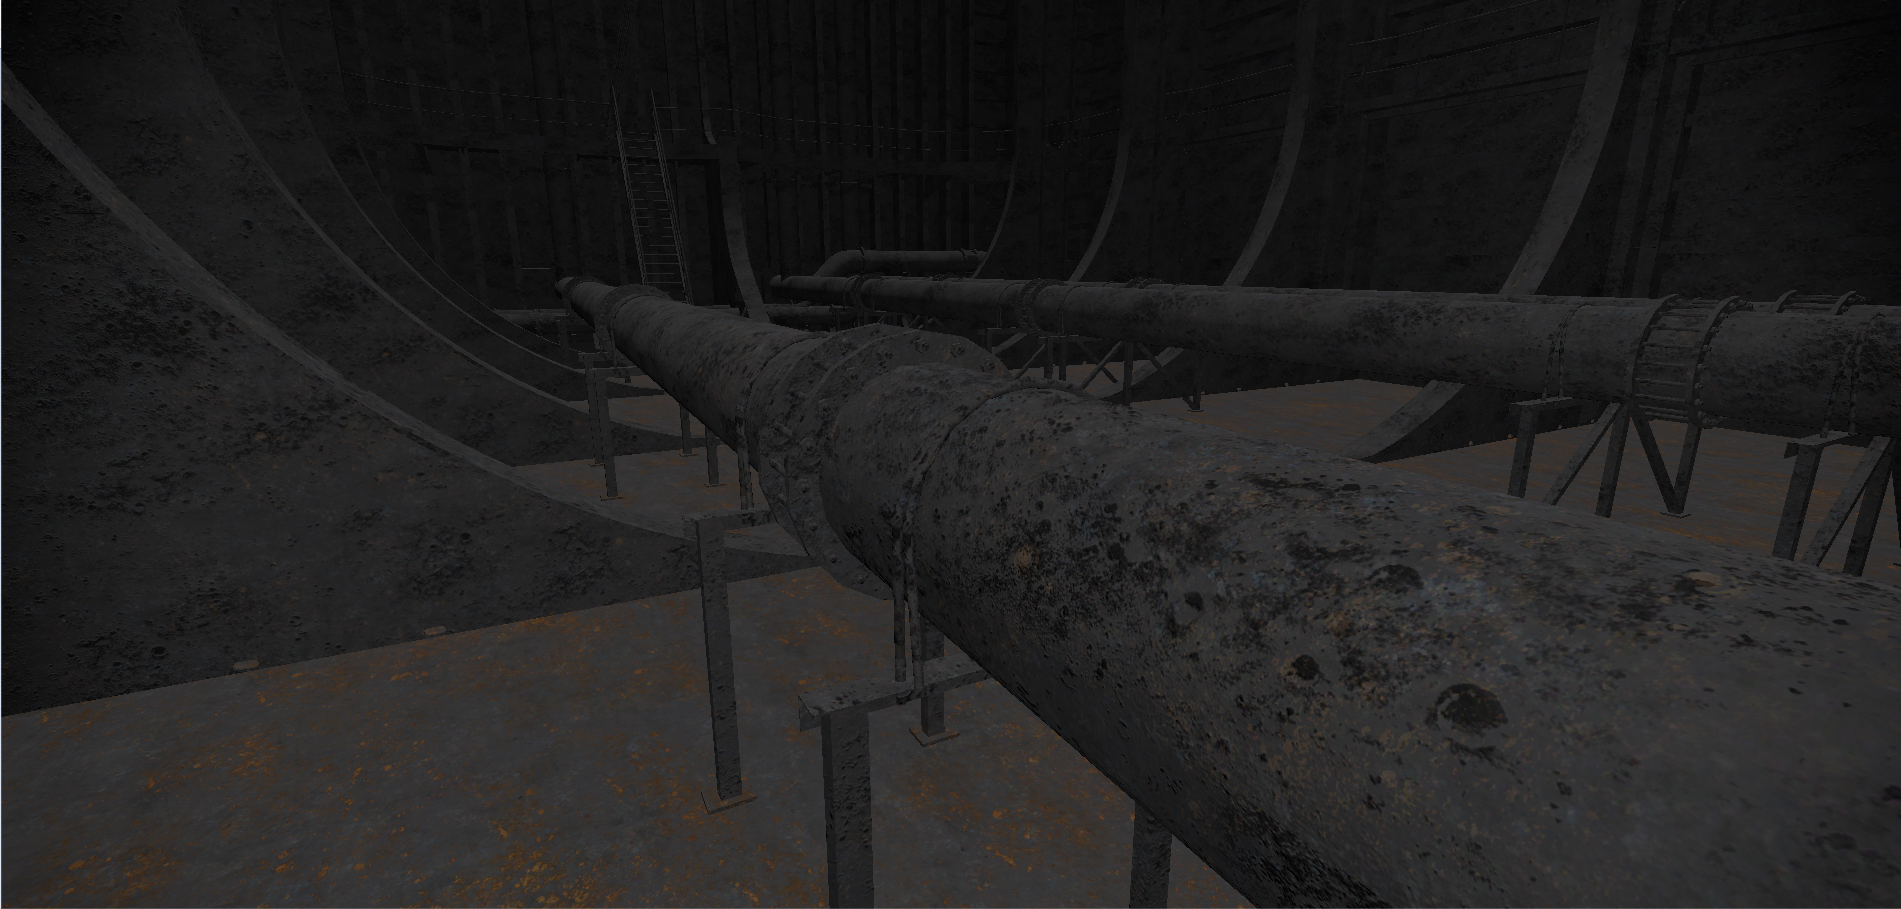
\includegraphics[width=\linewidth]{pictures/screenshots/annotation_visibility/invisible.png}
% 	\caption[Annotation invisible]{When selecting the "Invisible" option in the Annotation Visibility Submenu annotations are not visible and can not be interacted with.}
% 	\label{fig:invisible}
% \end{figure} 

\section{The Movement- and Rotation Controller}
\texttt{MovementController} and \texttt{RotationController} are script components of the MasterController, and relates to the movement and rotation of the user.










% Important child objects of MasterController include CameraRigs, which holds seperate camera rigs for either destop, oculus rift or htc vive usage, 
% WorldSpaceCanvas for drawing user interfaces in the game world, LeapMotionController for aspects related to the Leap Motion and
% GazePointerRing to enable the gazepointer ring when a virtual reality headset is used. These are all documented below.


